\documentclass[11pt,a4paper,fleqn]{article}
\usepackage{times}
\thispagestyle{empty}



\usepackage[T1]{fontenc}   % Silbentrennung

\usepackage[utf8x]{inputenc}
                                                                                                                             
\hyphenation{Acad-e-my}

\usepackage[bookmarks=true,bookmarksopen=true,%
breaklinks=true,%
draft=false,plainpages=false,hyperfootnotes=false,%
pdfauthor={Stefan Müller (Editor)},%
pdftitle={Proceedings of the 20th International Conference on Head-Driven Phrase Structure Grammar},%
pdfkeywords={HPSG}%,
pdftex=true%
%ps2pdf=true  %ohne diesen Treiber geht der Zeilenumbruch in URLs
]{hyperref}% for pdf files
\hypersetup{colorlinks=false, pdfborder={0 0 0}}

\usepackage{pdfpages}
\pdfinclusioncopyfonts=1

\newcommand\formatauthor[2]{\begin{tabular}[t]{@{}c@{}}
  {\LARGE#1\strut}\\
  {\small#2\strut}\\
  \rule{\dimexpr0.5\linewidth-1em}{0pt}
  \end{tabular}\xhfill\ignorespaces}
\newcommand\xhfill{\hspace{1em plus 1fill}}

\begin{document}

\begin{center}
{\Large
                {\bfseries Proceedings of the 20th International Conference on\par Head-Driven Phrase Structure Grammar\par}

                \vspace{8ex}

                     Freie Universit\"{a}t Berlin\\[\baselineskip]

                        Stefan M{\"u}ller (Editor)\\[\baselineskip]

                                2013\\[\baselineskip]

                          CSLI Publications\\[\baselineskip]

              http://csli-publications.stanford.edu/HPSG/2013 \\[4\baselineskip]

The papers are published under a \href{http://creativecommons.org/licenses/by/4.0/}{CC-BY license}:\\[3pt]
\href{http://creativecommons.org/licenses/by/4.0/}{http://creativecommons.org/licenses/by/4.0/}
}
\end{center}
\newpage
\tableofcontents

\newpage

\section{Editor's Note}
%% -*- coding:utf-8 -*-
The 20th International Conference on Head-Driven Phrase Structure Grammar (2013) was held at the
Freie Universität Berlin.

The conference featured 2 invited talks and 15 papers selected by the program committee 
(Emily M. Bender,
    Olivier Bonami,
    Bob Borsley,
    Rui Chaves,
    Berthold Crysmann,
    Kordula De Kuthy,
    Elisabet Engdahl,
    Daniel Flickinger,
    Jong-Bok Kim,
    Jean-Pierre Koenig,
    Valia Kordoni,
    Anna Kupsc,
    Robert Levine,
    Nurit Melnik,
    Stefan Müller,
    Tsuneko Nakazawa,
    Gerald Penn,
    Adam Przepiórkowski,
    Frank Richter,
    Louisa Sadler,
    Ivan Sag,
    Manfred Sailer,
    Jesse Tseng (chair),
    Frank Van Eynde,
    Gert Webelhuth,
    Stephen Wechsler,
    Shuichi Yatabe,
    Eun-Jung Yoo).

A tutorial \emph{Linguistic Research with Large Annotated Web Corpora} by Felix Bild\-hauer
and Roland Schäfer and a workshop about \emph{Progress in Linguistics}
were attached to the conference. The workshop program was put together by Stefan Müller and consisted of
invited talks only.

% wie viele?
%In total there were 27  submissions to the conference and 0 submissions to the workshop.
We want to thank the respective program committees for putting this nice program together.

Thanks go to Stefan Müller (chair), Viola Auermann, Lea Helmers, and Jakob Maché, who were
in charge of local arrangements.
 
The conference was supported by a grant from the Deutsche Forschungsgemeinschaft to Stefan Müller (MU 2822/7-1).

As in the past years the contributions to the conference proceedings are based on the five page abstract
that was reviewed by the respective program committees, but there is no additional reviewing of the
longer contribution to the proceedings.
To ensure easy access and fast publication we have chosen an electronic format.

The proceedings include all the papers except those by  Farell Ackerman, Rob Malouf, and John Moore,
Tibor Kiss, Takafumi Maekawa, Gereon Müller, Stefan Müller (workshop), Andreas Pankau, Frank
Richter, Anatol Stefanowitsch, and Nigel Vincent.



\newpage
\part{Contributions to the Main Conference}
\thispagestyle{empty}
\newpage
        \setcounter{page}{6}
        \phantomsection
        \addcontentsline{toc}{section}{Mansour Alotaibi, Robert D. Borsley: Gaps and Resumptive Pronouns in {Modern Standard Arabic}}
\thispagestyle{empty}

\begin{center}
  {\huge\bfseries Gaps and Resumptive Pronouns in {Modern Standard Arabic}\par}

  \bigskip

~\\
\begingroup
\setlength{\leftskip}{0pt plus 1fill}
\setlength{\rightskip}{0pt plus 1fill}
\setlength{\parindent}{0pt}
\setlength{\parfillskip}{0pt}
  \formatauthor{Mansour Alotaibi}{\begin{tabular}{@{}c@{}}University of Essex, Salman bin Abdulaziz University\end{tabular}}
\formatauthor{Robert D. Borsley}{\begin{tabular}{@{}c@{}}University of Essex\end{tabular}}

\par\endgroup

  \vspace*{8ex}

  Proceedings of the 20th International Conference on\par Head-Driven Phrase Structure Grammar

  \bigskip

  Freie Universit\"{a}t Berlin

  \medskip

  Stefan Müller (Editor)

  \medskip

  2013

  \medskip

  CSLI Publications

  \medskip

  pages 6--26

  \medskip

  \url{http://csli-publications.stanford.edu/HPSG/2013}
\end{center}
\vfill

\noindent



\vfill
\noindent
% APA Style
Alotaibi, Mansour, \& Borsley, Robert D. 2013. Gaps and Resumptive Pronouns in {Modern Standard Arabic}. In Müller, Stefan (Ed.), \emph{{Proceedings of the 20th International Conference on Head-Driven Phrase Structure Grammar, Freie Universit\"{a}t Berlin}}, 6--26. Stanford,
CA: CSLI Publications. \hfill\href{http://creativecommons.org/licenses/by/4.0/}{\includegraphics[height=.75em]{Includes/ccby.eps}}

\newpage
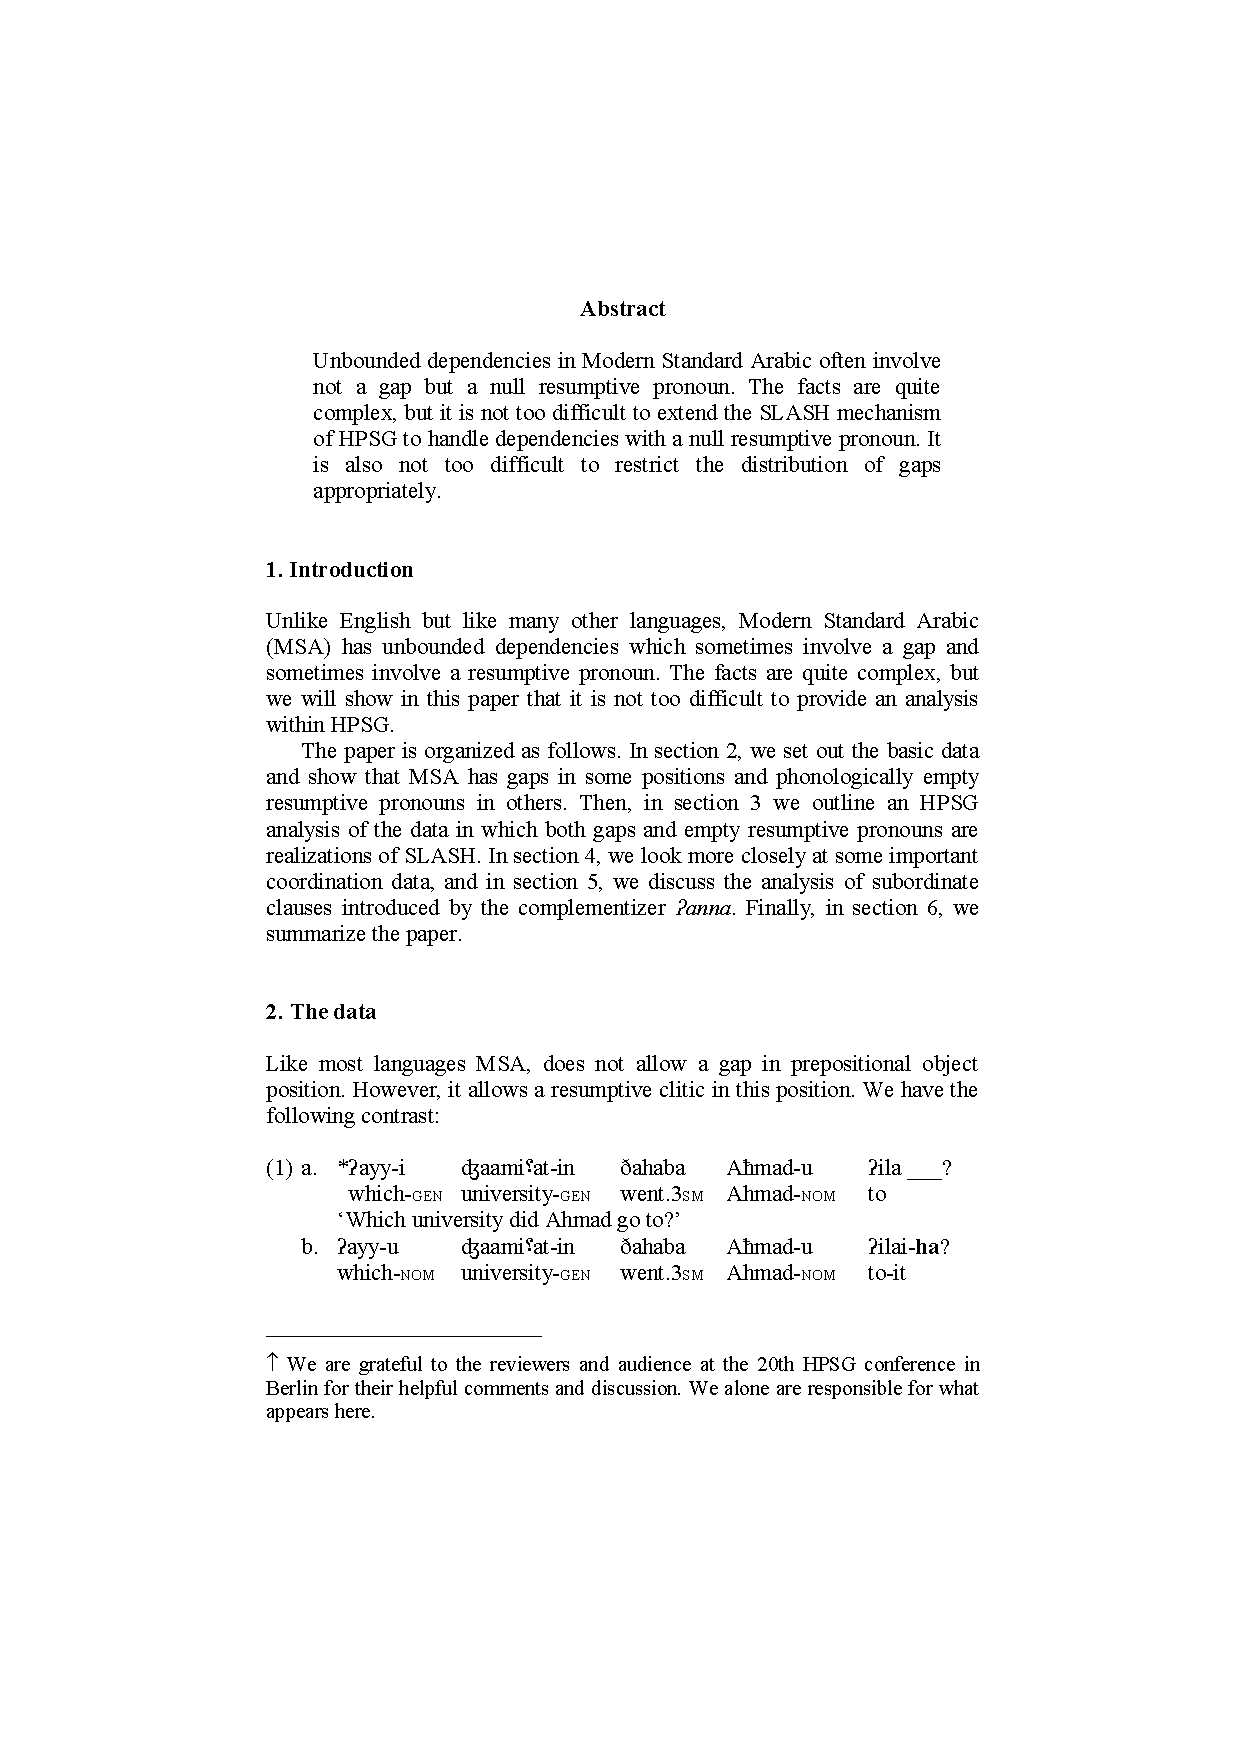
\includepdf[pages=-,pagecommand=\thispagestyle{plain}]{Includes/alotaibi-borsley.pdf}
        \setcounter{page}{27}
        \phantomsection
        \addcontentsline{toc}{section}{Olivier Bonami, Berthold Crysmann: Morphotactics in an Information-Based Model of Realisational Morphology}
\thispagestyle{empty}

\begin{center}
  {\huge\bfseries Morphotactics in an Information-Based Model of Realisational Morphology\par}

  \bigskip

~\\
\begingroup
\setlength{\leftskip}{0pt plus 1fill}
\setlength{\rightskip}{0pt plus 1fill}
\setlength{\parindent}{0pt}
\setlength{\parfillskip}{0pt}
  \formatauthor{Olivier Bonami}{\begin{tabular}{@{}c@{}}Université Paris-Sorbonne \\ Institut universitaire de France \\ LLF (UMR 7110)\end{tabular}}
\formatauthor{Berthold Crysmann}{\begin{tabular}{@{}c@{}}CNRS \\  LLF  (UMR 7110)\end{tabular}}

\par\endgroup

  \vspace*{8ex}

  Proceedings of the 20th International Conference on\par Head-Driven Phrase Structure Grammar

  \bigskip

  Freie Universit\"{a}t Berlin

  \medskip

  Stefan Müller (Editor)

  \medskip

  2013

  \medskip

  CSLI Publications

  \medskip

  pages 27--47

  \medskip

  \url{http://csli-publications.stanford.edu/HPSG/2013}
\end{center}
\vfill

\noindent



\vfill
\noindent
% APA Style
Bonami, Olivier, \& Crysmann, Berthold. 2013. Morphotactics in an Information-Based Model of Realisational Morphology. In Müller, Stefan (Ed.), \emph{{Proceedings of the 20th International Conference on Head-Driven Phrase Structure Grammar, Freie Universit\"{a}t Berlin}}, 27--47. Stanford,
CA: CSLI Publications. \hfill\href{http://creativecommons.org/licenses/by/4.0/}{\includegraphics[height=.75em]{Includes/ccby.eps}}

\newpage
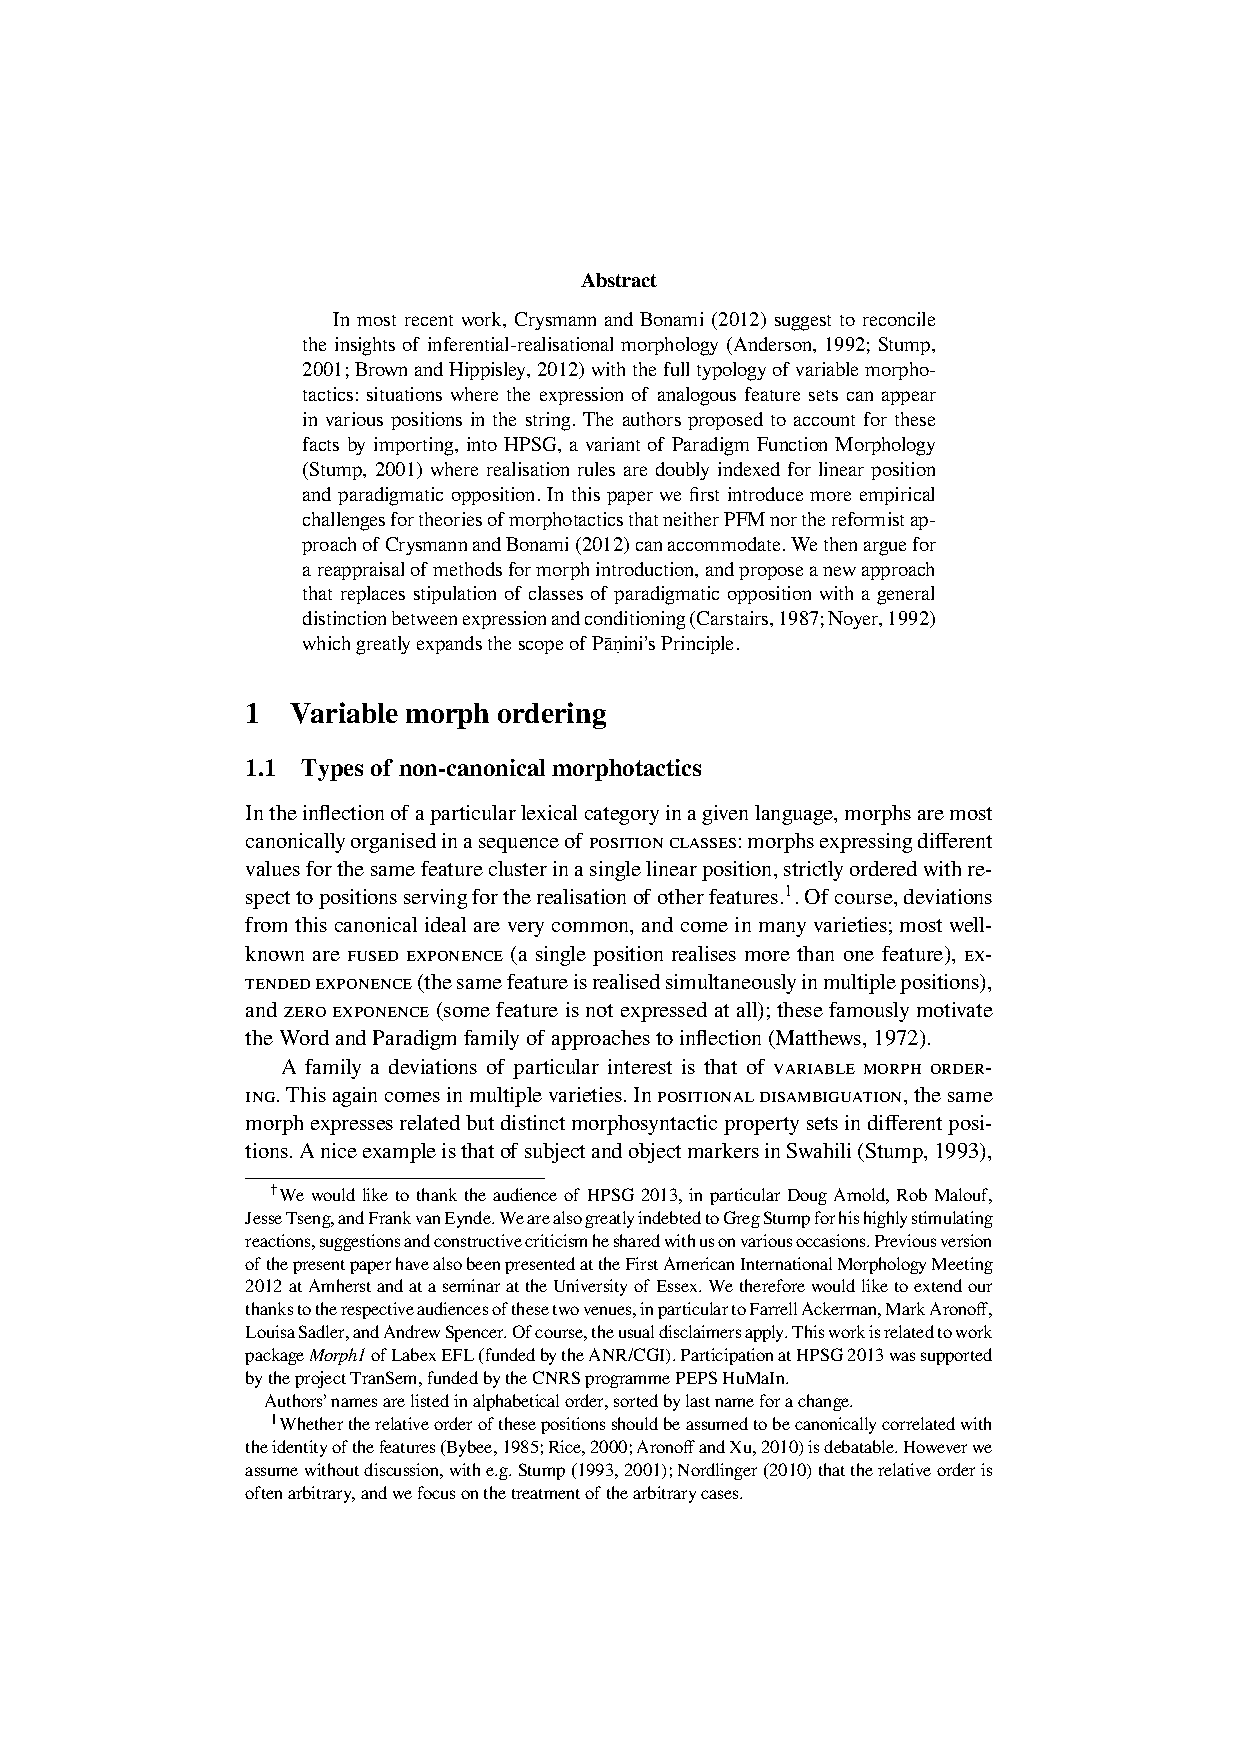
\includepdf[pages=-,pagecommand=\thispagestyle{plain}]{Includes/bonami-crysmann.pdf}
        \setcounter{page}{48}
        \phantomsection
        \addcontentsline{toc}{section}{Michael Hahn: Word Order Variation in Khoekhoe}
\thispagestyle{empty}

\begin{center}
  {\huge\bfseries Word Order Variation in Khoekhoe\par}

  \bigskip

~\\
\begingroup
\setlength{\leftskip}{0pt plus 1fill}
\setlength{\rightskip}{0pt plus 1fill}
\setlength{\parindent}{0pt}
\setlength{\parfillskip}{0pt}
  \formatauthor{Michael Hahn}{\begin{tabular}{@{}c@{}}University of Tübingen\end{tabular}}

\par\endgroup

  \vspace*{8ex}

  Proceedings of the 20th International Conference on\par Head-Driven Phrase Structure Grammar

  \bigskip

  Freie Universit\"{a}t Berlin

  \medskip

  Stefan Müller (Editor)

  \medskip

  2013

  \medskip

  CSLI Publications

  \medskip

  pages 48--68

  \medskip

  \url{http://csli-publications.stanford.edu/HPSG/2013}
\end{center}
\vfill

\noindent



\vfill
\noindent
% APA Style
Hahn, Michael. 2013. Word Order Variation in Khoekhoe. In Müller, Stefan (Ed.), \emph{{Proceedings of the 20th International Conference on Head-Driven Phrase Structure Grammar, Freie Universit\"{a}t Berlin}}, 48--68. Stanford,
CA: CSLI Publications. \hfill\href{http://creativecommons.org/licenses/by/4.0/}{\includegraphics[height=.75em]{Includes/ccby.eps}}

\newpage
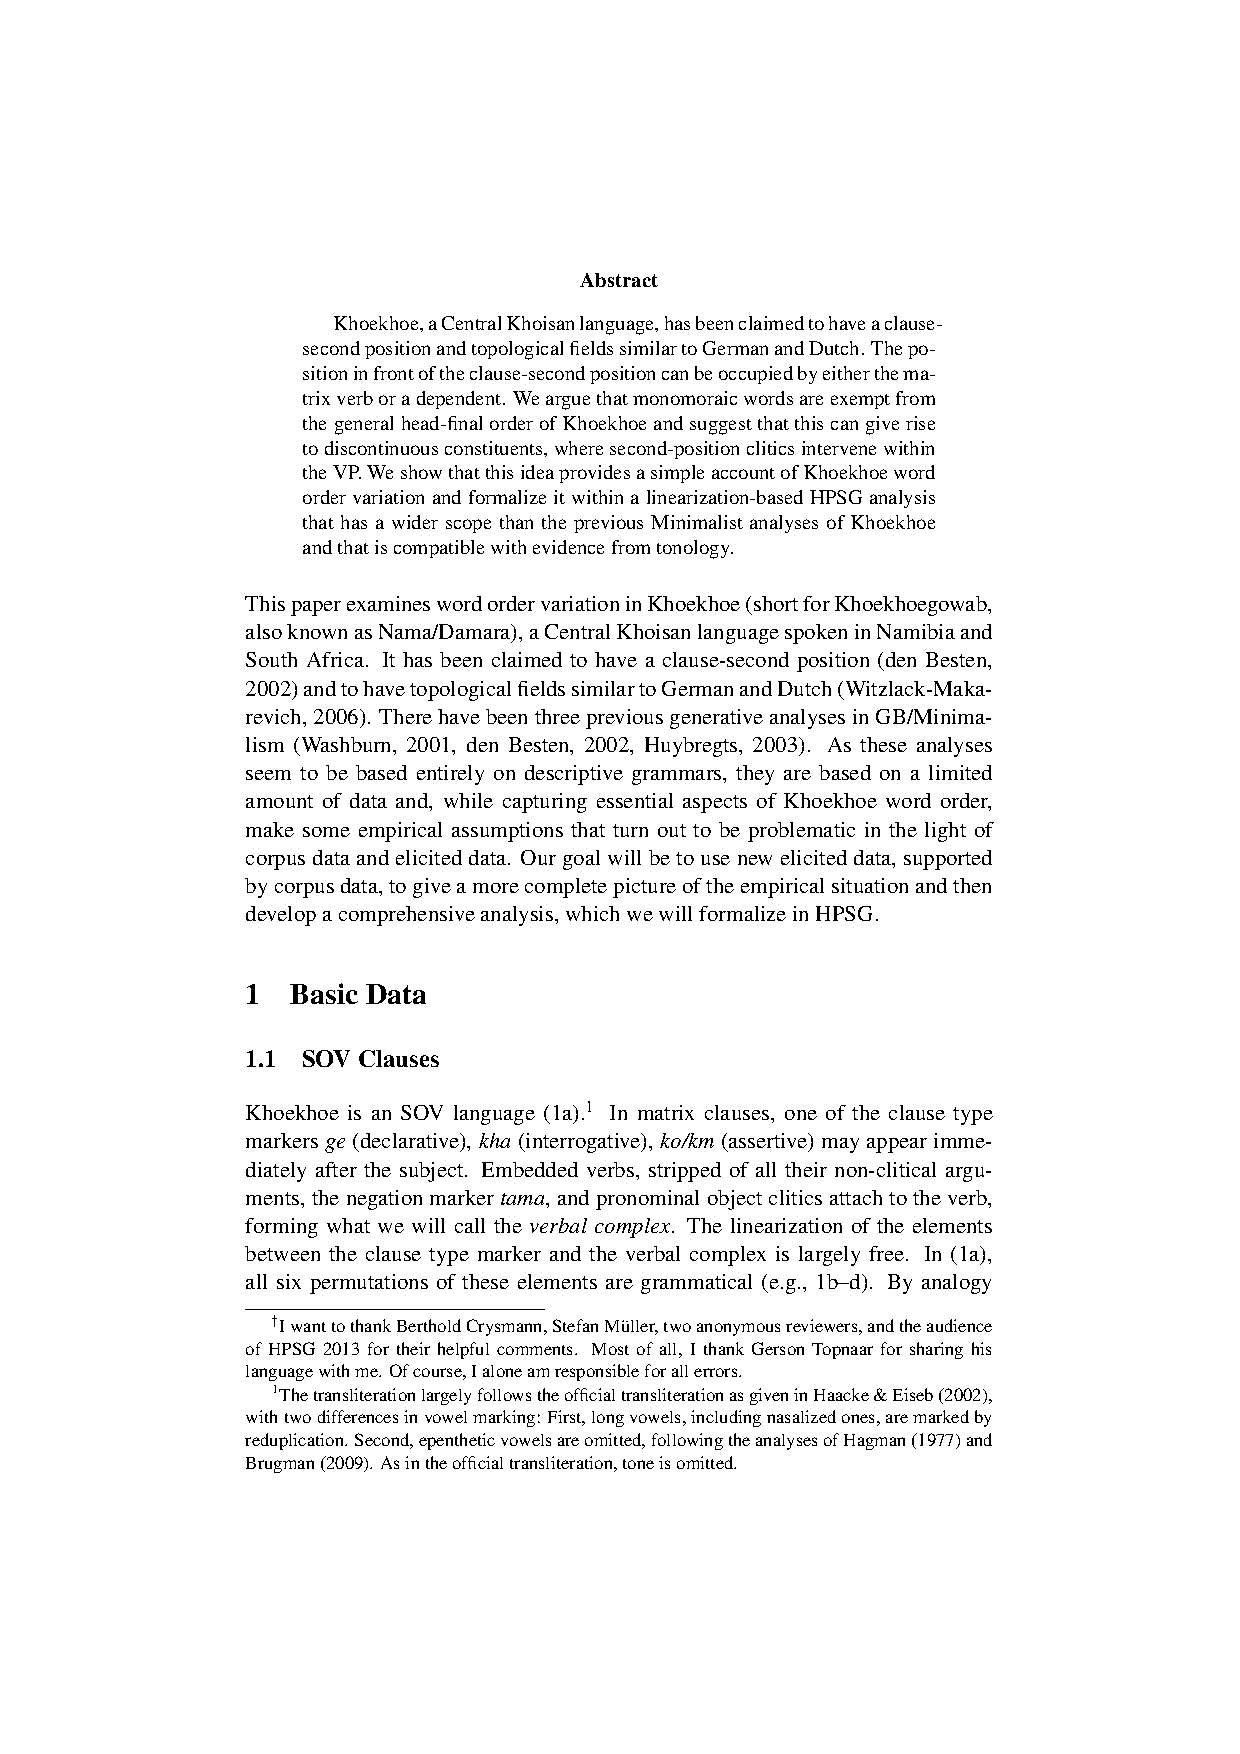
\includepdf[pages=-,pagecommand=\thispagestyle{plain}]{Includes/hahn.pdf}
        \setcounter{page}{69}
        \phantomsection
        \addcontentsline{toc}{section}{Petter Haugereid, Nurit Melnik, Shuly Wintner: Nonverbal Predicates in {Modern Hebrew}}
\thispagestyle{empty}

\begin{center}
  {\huge\bfseries Nonverbal Predicates in {Modern Hebrew}\par}

  \bigskip

~\\
\begingroup
\setlength{\leftskip}{0pt plus 1fill}
\setlength{\rightskip}{0pt plus 1fill}
\setlength{\parindent}{0pt}
\setlength{\parfillskip}{0pt}
  \formatauthor{Petter Haugereid}{\begin{tabular}{@{}c@{}}University of Bergen \\ The Open University of Israel \\ University of Haifa\end{tabular}}
\formatauthor{Nurit Melnik}{\begin{tabular}{@{}c@{}}The Open University of Israel\end{tabular}}
\formatauthor{Shuly Wintner}{\begin{tabular}{@{}c@{}}University of Haifa\end{tabular}}

\par\endgroup

  \vspace*{8ex}

  Proceedings of the 20th International Conference on\par Head-Driven Phrase Structure Grammar

  \bigskip

  Freie Universit\"{a}t Berlin

  \medskip

  Stefan Müller (Editor)

  \medskip

  2013

  \medskip

  CSLI Publications

  \medskip

  pages 69--89

  \medskip

  \url{http://csli-publications.stanford.edu/HPSG/2013}
\end{center}
\vfill

\noindent



\vfill
\noindent
% APA Style
Haugereid, Petter, Melnik, Nurit, \& Wintner, Shuly. 2013. Nonverbal Predicates in {Modern Hebrew}. In Müller, Stefan (Ed.), \emph{{Proceedings of the 20th International Conference on Head-Driven Phrase Structure Grammar, Freie Universit\"{a}t Berlin}}, 69--89. Stanford,
CA: CSLI Publications. \hfill\href{http://creativecommons.org/licenses/by/4.0/}{\includegraphics[height=.75em]{Includes/ccby.eps}}

\newpage
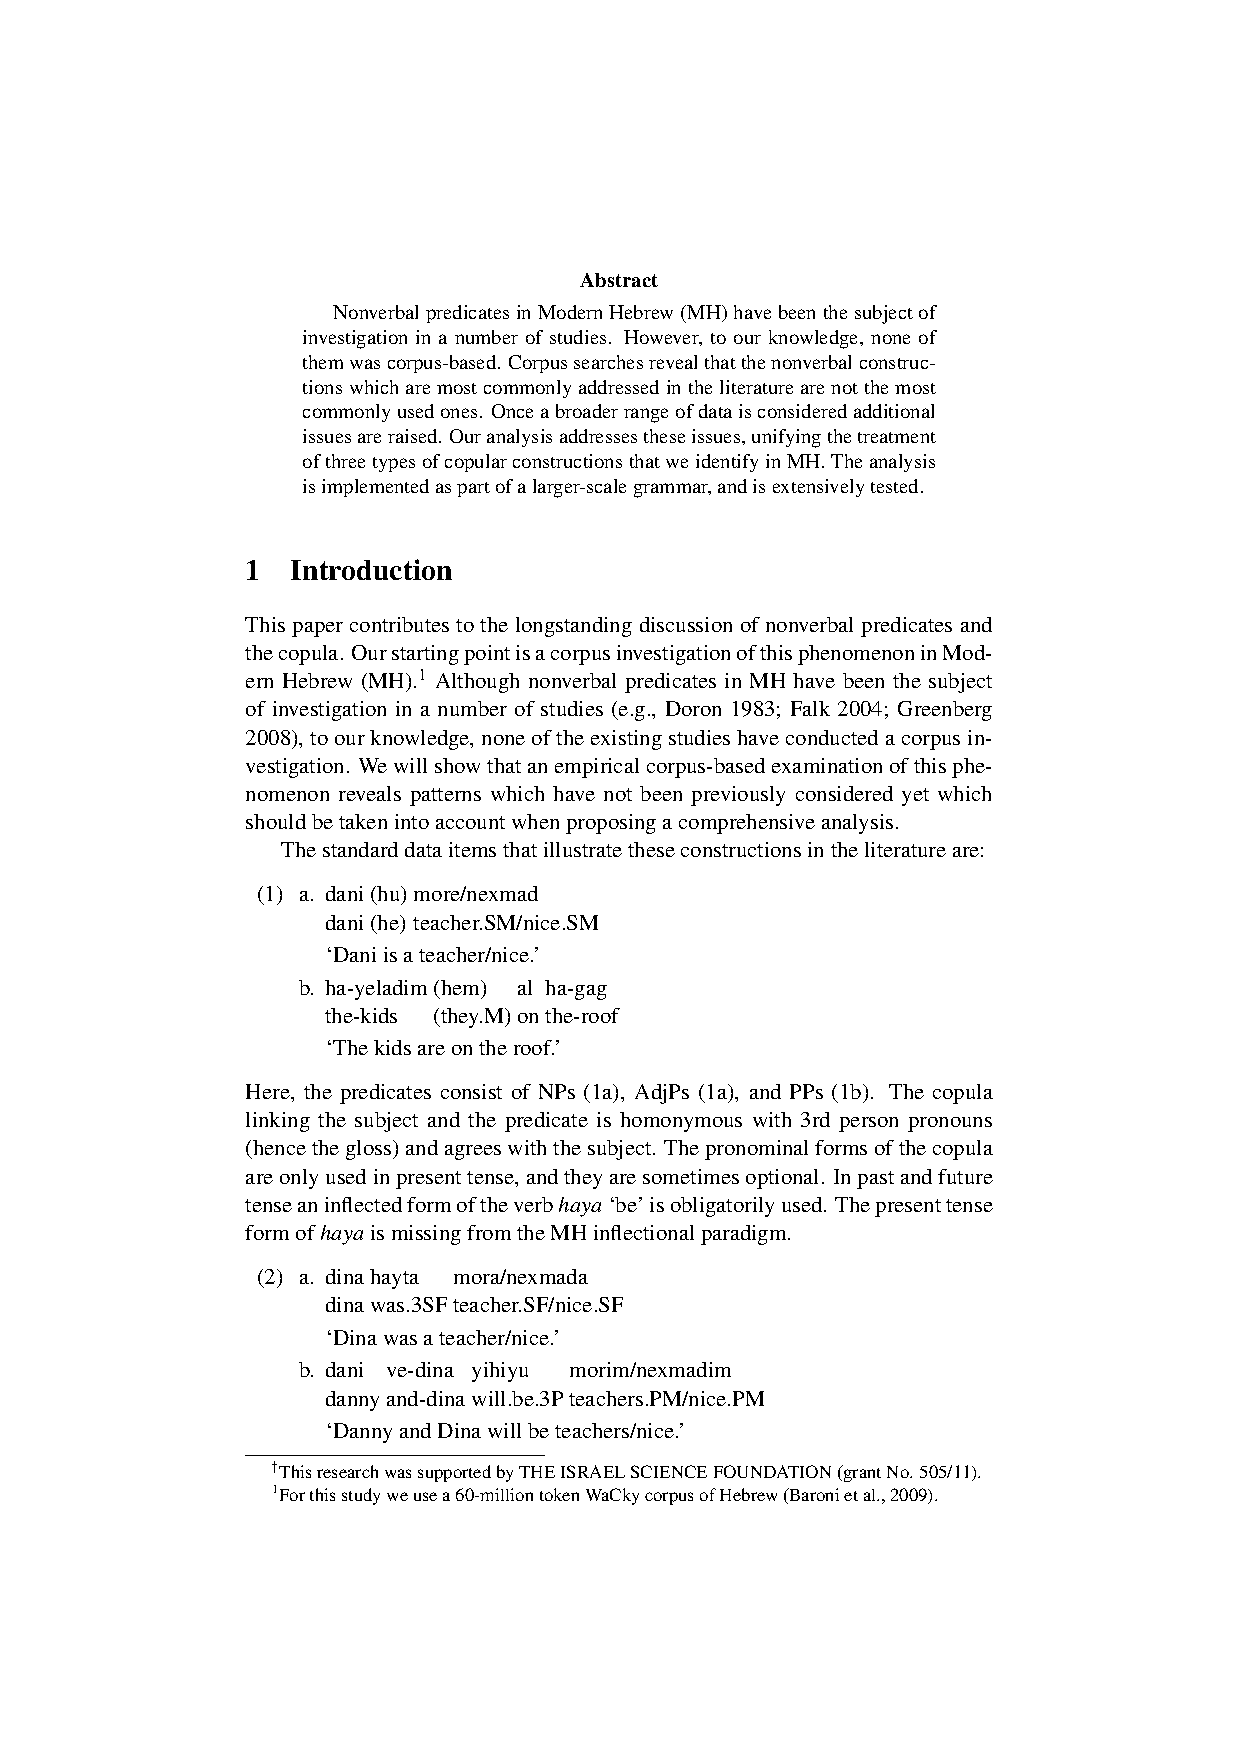
\includepdf[pages=-,pagecommand=\thispagestyle{plain}]{Includes/hmw.pdf}
        \setcounter{page}{90}
        \phantomsection
        \addcontentsline{toc}{section}{Anke Holler: Reanalyzing {German} Correlative \emph{es}}
\thispagestyle{empty}

\begin{center}
  {\huge\bfseries Reanalyzing {German} Correlative \emph{es}\par}

  \bigskip

~\\
\begingroup
\setlength{\leftskip}{0pt plus 1fill}
\setlength{\rightskip}{0pt plus 1fill}
\setlength{\parindent}{0pt}
\setlength{\parfillskip}{0pt}
  \formatauthor{Anke Holler}{\begin{tabular}{@{}c@{}}University of Göttingen\end{tabular}}

\par\endgroup

  \vspace*{8ex}

  Proceedings of the 20th International Conference on\par Head-Driven Phrase Structure Grammar

  \bigskip

  Freie Universit\"{a}t Berlin

  \medskip

  Stefan Müller (Editor)

  \medskip

  2013

  \medskip

  CSLI Publications

  \medskip

  pages 90--109

  \medskip

  \url{http://csli-publications.stanford.edu/HPSG/2013}
\end{center}
\vfill

\noindent



\vfill
\noindent
% APA Style
Holler, Anke. 2013. Reanalyzing {German} Correlative \emph{es}. In Müller, Stefan (Ed.), \emph{{Proceedings of the 20th International Conference on Head-Driven Phrase Structure Grammar, Freie Universit\"{a}t Berlin}}, 90--109. Stanford,
CA: CSLI Publications. \hfill\href{http://creativecommons.org/licenses/by/4.0/}{\includegraphics[height=.75em]{Includes/ccby.eps}}

\newpage
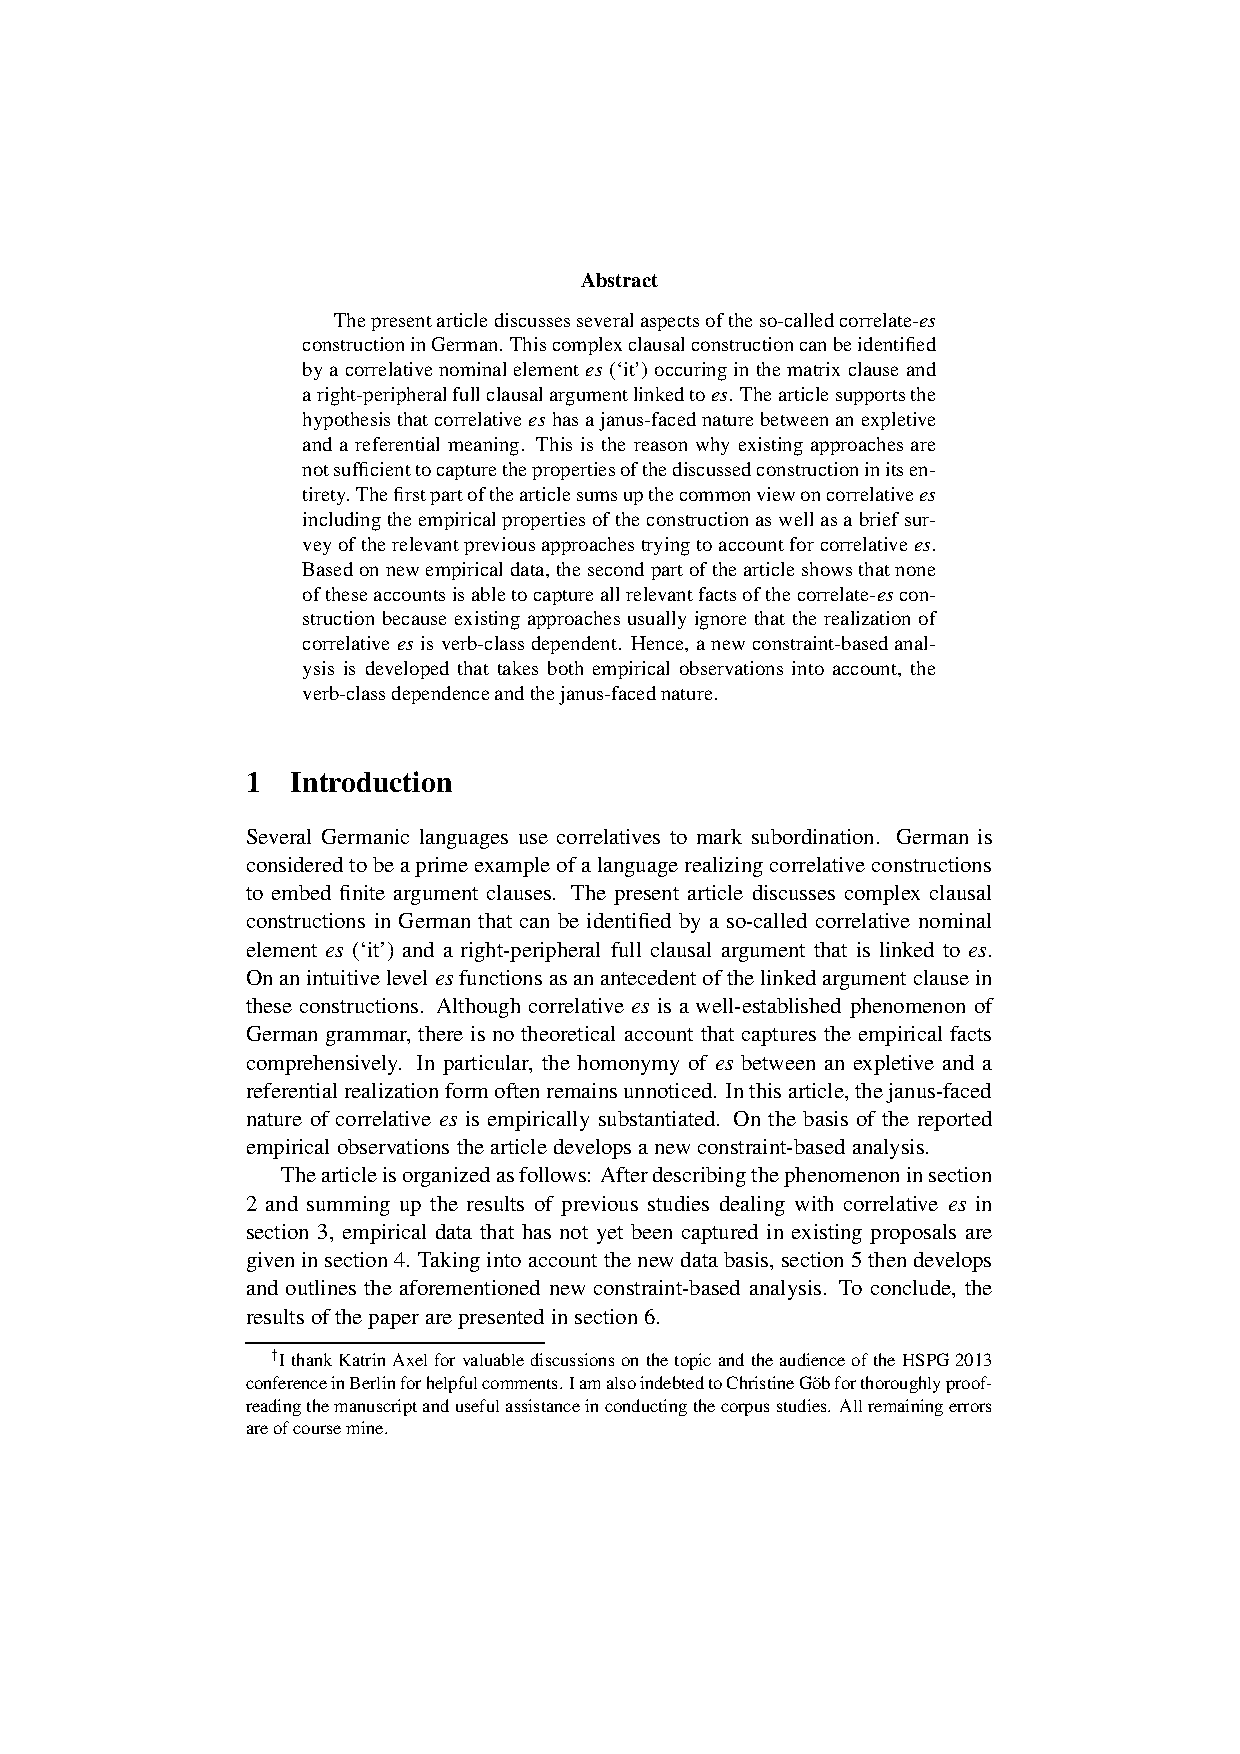
\includepdf[pages=-,pagecommand=\thispagestyle{plain}]{Includes/holler.pdf}
        \setcounter{page}{110}
        \phantomsection
        \addcontentsline{toc}{section}{Dawei Jin: Information Structure Constraints and Complex NP Islands in {Chinese}}
\thispagestyle{empty}

\begin{center}
  {\huge\bfseries Information Structure Constraints and Complex NP Islands in {Chinese}\par}

  \bigskip

~\\
\begingroup
\setlength{\leftskip}{0pt plus 1fill}
\setlength{\rightskip}{0pt plus 1fill}
\setlength{\parindent}{0pt}
\setlength{\parfillskip}{0pt}
  \formatauthor{Dawei Jin}{\begin{tabular}{@{}c@{}}University at Buffalo, SUNY\end{tabular}}

\par\endgroup

  \vspace*{8ex}

  Proceedings of the 20th International Conference on\par Head-Driven Phrase Structure Grammar

  \bigskip

  Freie Universit\"{a}t Berlin

  \medskip

  Stefan Müller (Editor)

  \medskip

  2013

  \medskip

  CSLI Publications

  \medskip

  pages 110--120

  \medskip

  \url{http://csli-publications.stanford.edu/HPSG/2013}
\end{center}
\vfill

\noindent



\vfill
\noindent
% APA Style
Jin, Dawei. 2013. Information Structure Constraints and Complex NP Islands in {Chinese}. In Müller, Stefan (Ed.), \emph{{Proceedings of the 20th International Conference on Head-Driven Phrase Structure Grammar, Freie Universit\"{a}t Berlin}}, 110--120. Stanford,
CA: CSLI Publications. \hfill\href{http://creativecommons.org/licenses/by/4.0/}{\includegraphics[height=.75em]{Includes/ccby.eps}}

\newpage
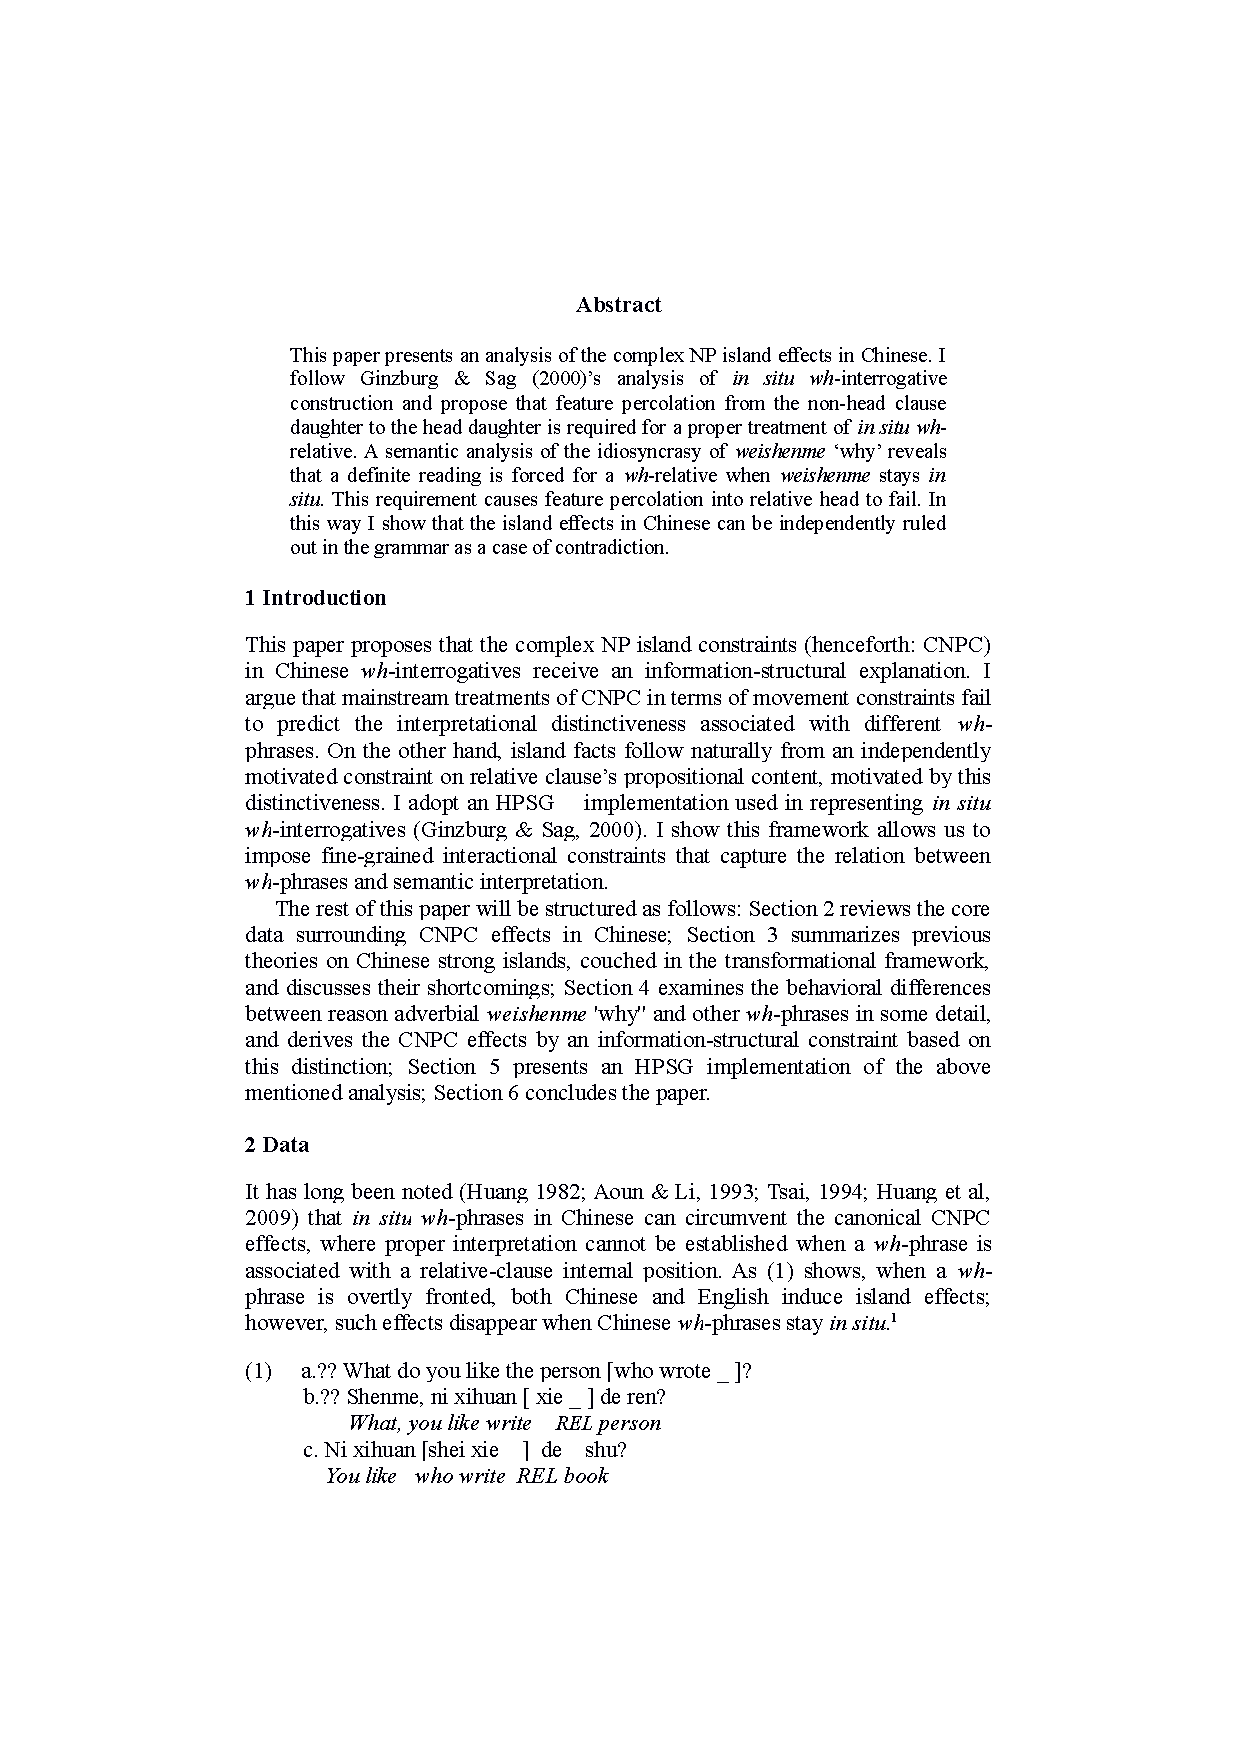
\includepdf[pages=-,pagecommand=\thispagestyle{plain}]{Includes/jin.pdf}
        \setcounter{page}{121}
        \phantomsection
        \addcontentsline{toc}{section}{Philip Miller: Usage Preferences: The Case of the {English} Verbal Anaphor \emph{do so}}
\thispagestyle{empty}

\begin{center}
  {\huge\bfseries Usage Preferences: The Case of the {English} Verbal Anaphor \emph{do so}\par}

  \bigskip

~\\
\begingroup
\setlength{\leftskip}{0pt plus 1fill}
\setlength{\rightskip}{0pt plus 1fill}
\setlength{\parindent}{0pt}
\setlength{\parfillskip}{0pt}
  \formatauthor{Philip Miller}{\begin{tabular}{@{}c@{}}EA 3967 CLILLAC-ARP, Université Paris Diderot\end{tabular}}

\par\endgroup

  \vspace*{8ex}

  Proceedings of the 20th International Conference on\par Head-Driven Phrase Structure Grammar

  \bigskip

  Freie Universit\"{a}t Berlin

  \medskip

  Stefan Müller (Editor)

  \medskip

  2013

  \medskip

  CSLI Publications

  \medskip

  pages 121--139

  \medskip

  \url{http://csli-publications.stanford.edu/HPSG/2013}
\end{center}
\vfill

\noindent



\vfill
\noindent
% APA Style
Miller, Philip. 2013. Usage Preferences: The Case of the {English} Verbal Anaphor \emph{do so}. In Müller, Stefan (Ed.), \emph{{Proceedings of the 20th International Conference on Head-Driven Phrase Structure Grammar, Freie Universit\"{a}t Berlin}}, 121--139. Stanford,
CA: CSLI Publications. \hfill\href{http://creativecommons.org/licenses/by/4.0/}{\includegraphics[height=.75em]{Includes/ccby.eps}}

\newpage
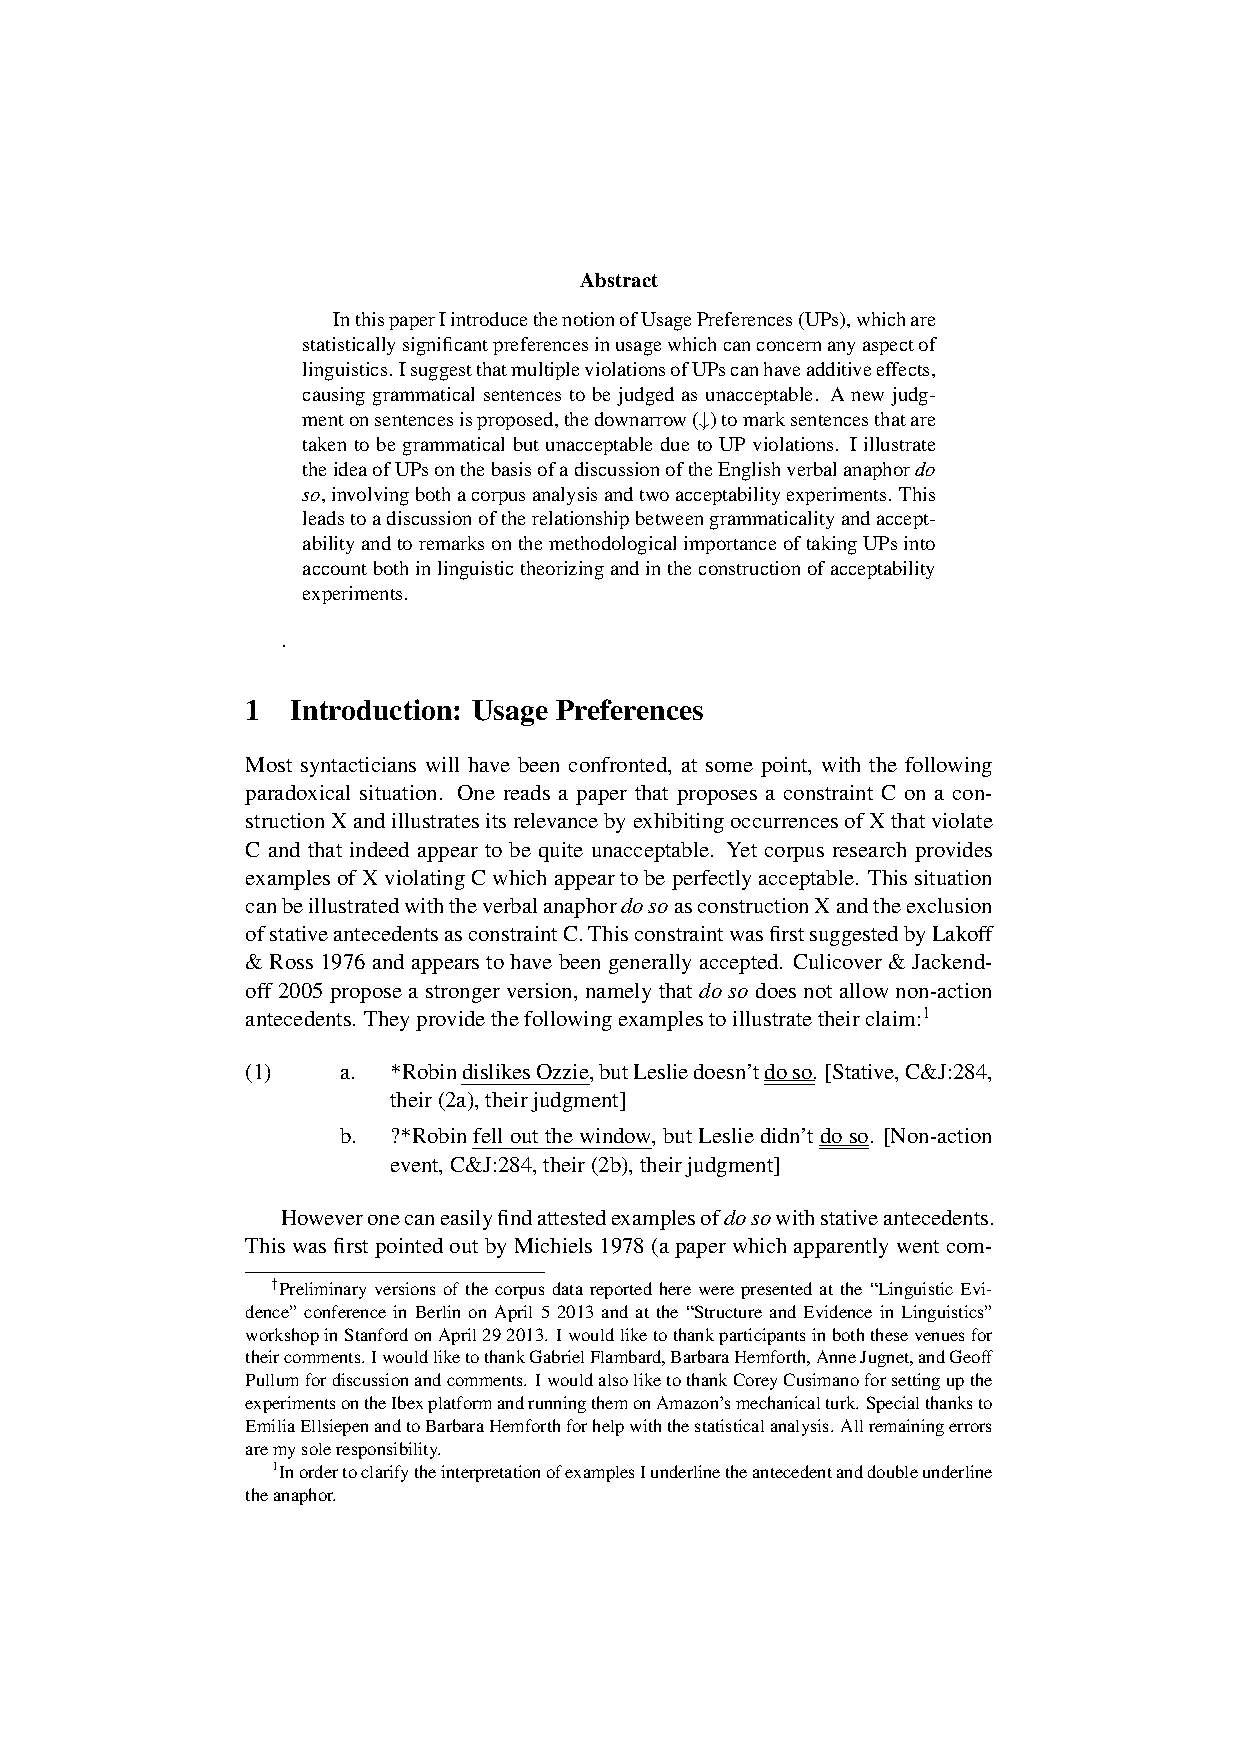
\includepdf[pages=-,pagecommand=\thispagestyle{plain}]{Includes/miller.pdf}
        \setcounter{page}{140}
        \phantomsection
        \addcontentsline{toc}{section}{Stefan M{\"u}ller, Bjarne {\O}rsnes: Passive in {Danish}, {English}, and {German}}
\thispagestyle{empty}

\begin{center}
  {\huge\bfseries Passive in {Danish}, {English}, and {German}\par}

  \bigskip

~\\
\begingroup
\setlength{\leftskip}{0pt plus 1fill}
\setlength{\rightskip}{0pt plus 1fill}
\setlength{\parindent}{0pt}
\setlength{\parfillskip}{0pt}
  \formatauthor{Stefan Müller}{\begin{tabular}{@{}c@{}}Freie Universität Berlin\end{tabular}}
\formatauthor{Bjarne Ørsnes}{\begin{tabular}{@{}c@{}}Freie Universität Berlin\end{tabular}}

\par\endgroup

  \vspace*{8ex}

  Proceedings of the 20th International Conference on\par Head-Driven Phrase Structure Grammar

  \bigskip

  Freie Universit\"{a}t Berlin

  \medskip

  Stefan Müller (Editor)

  \medskip

  2013

  \medskip

  CSLI Publications

  \medskip

  pages 140--160

  \medskip

  \url{http://csli-publications.stanford.edu/HPSG/2013}
\end{center}
\vfill

\noindent



\vfill
\noindent
% APA Style
Müller, Stefan, \& Ørsnes, Bjarne. 2013. Passive in {Danish}, {English}, and {German}. In Müller, Stefan (Ed.), \emph{{Proceedings of the 20th International Conference on Head-Driven Phrase Structure Grammar, Freie Universit\"{a}t Berlin}}, 140--160. Stanford,
CA: CSLI Publications. \hfill\href{http://creativecommons.org/licenses/by/4.0/}{\includegraphics[height=.75em]{Includes/ccby.eps}}

\newpage
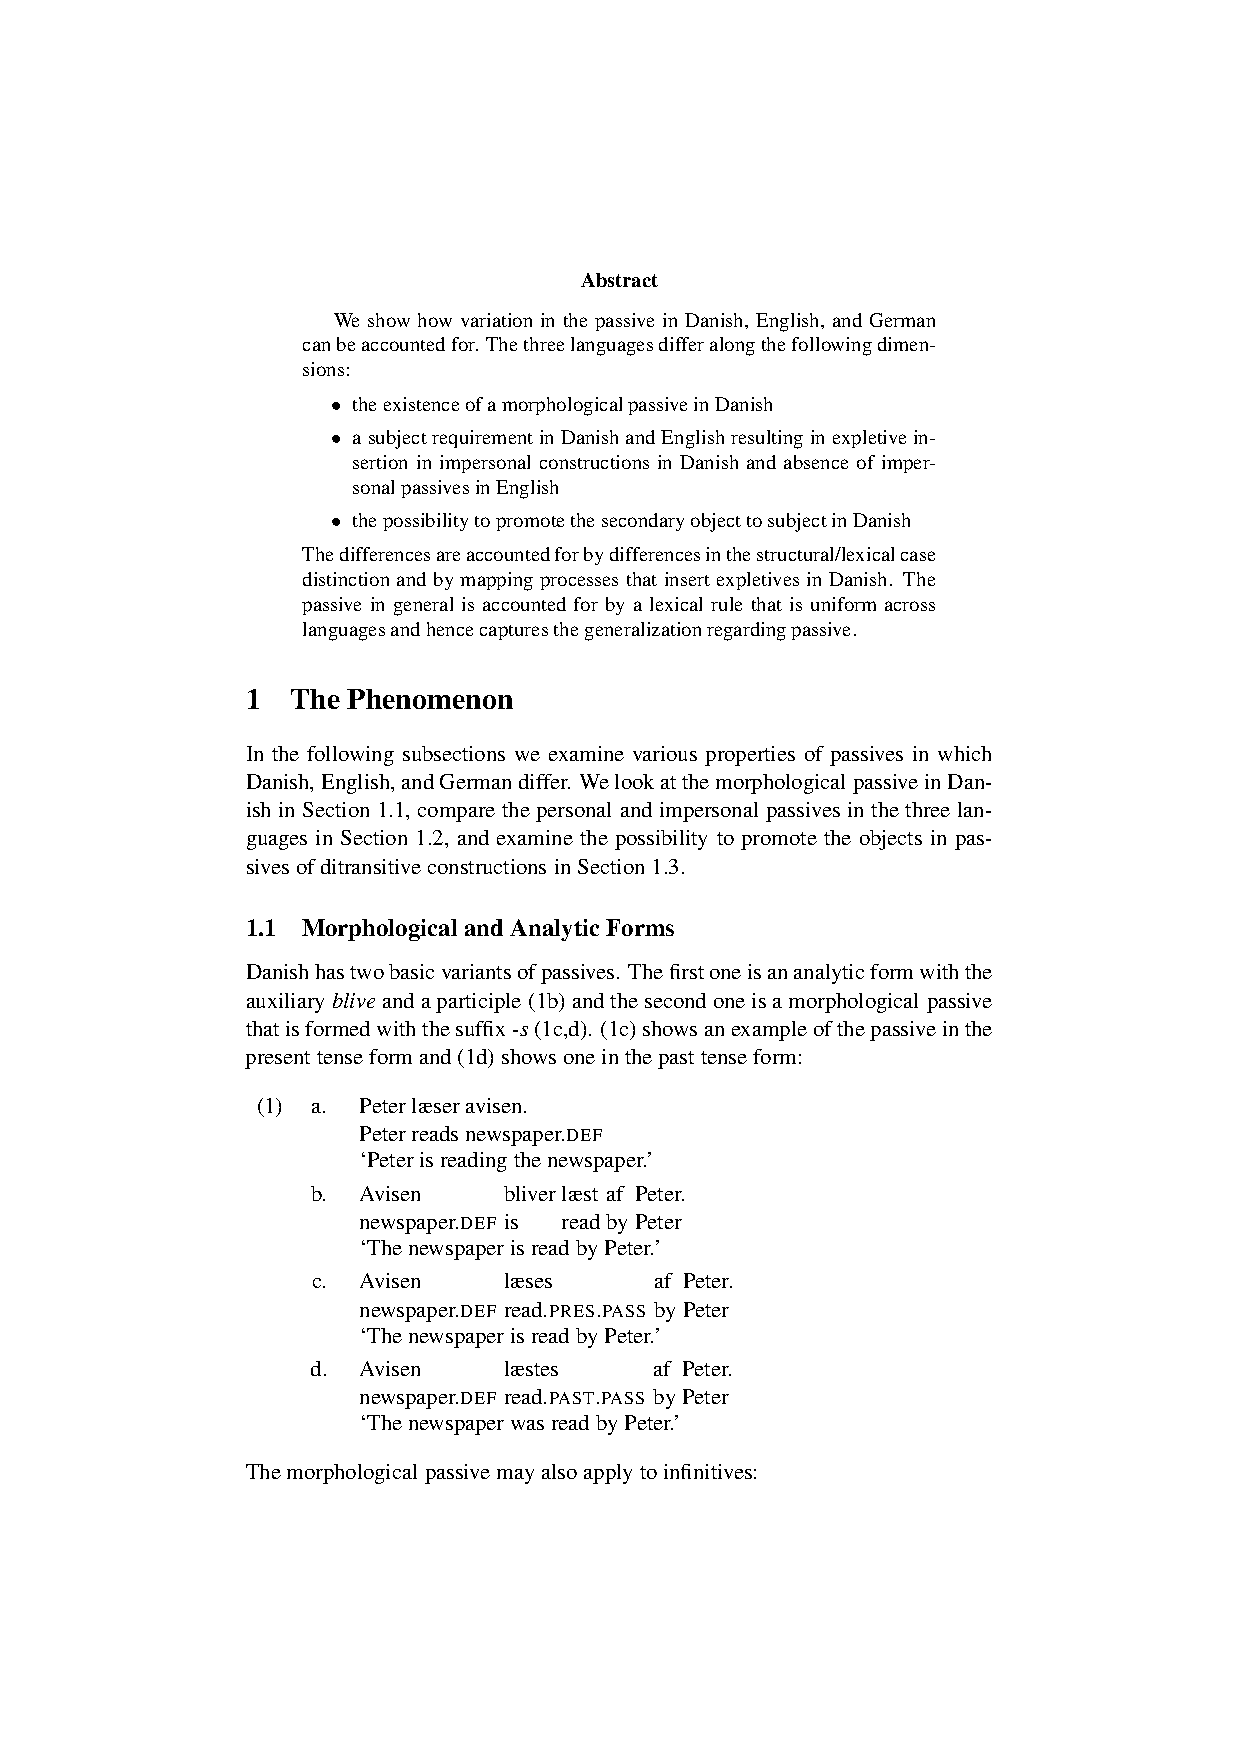
\includepdf[pages=-,pagecommand=\thispagestyle{plain}]{Includes/mueller-oersnes.pdf}
        \setcounter{page}{161}
        \phantomsection
        \addcontentsline{toc}{section}{Adam Przepi{\'o}rkowski: The Syntax of Distance Distributivity in {Polish}: Preserving Generalisations with Weak Heads}
\thispagestyle{empty}

\begin{center}
  {\huge\bfseries The Syntax of Distance Distributivity in {Polish}: Preserving Generalisations with Weak Heads\par}

  \bigskip

~\\
\begingroup
\setlength{\leftskip}{0pt plus 1fill}
\setlength{\rightskip}{0pt plus 1fill}
\setlength{\parindent}{0pt}
\setlength{\parfillskip}{0pt}
  \formatauthor{Adam Przepiórkowski}{\begin{tabular}{@{}c@{}}Institute of Computer Science, Polish Academy of Sciences\end{tabular}}

\par\endgroup

  \vspace*{8ex}

  Proceedings of the 20th International Conference on\par Head-Driven Phrase Structure Grammar

  \bigskip

  Freie Universit\"{a}t Berlin

  \medskip

  Stefan Müller (Editor)

  \medskip

  2013

  \medskip

  CSLI Publications

  \medskip

  pages 161--181

  \medskip

  \url{http://csli-publications.stanford.edu/HPSG/2013}
\end{center}
\vfill

\noindent



\vfill
\noindent
% APA Style
Przepiórkowski, Adam. 2013. The Syntax of Distance Distributivity in {Polish}: Preserving Generalisations with Weak Heads. In Müller, Stefan (Ed.), \emph{{Proceedings of the 20th International Conference on Head-Driven Phrase Structure Grammar, Freie Universit\"{a}t Berlin}}, 161--181. Stanford,
CA: CSLI Publications. \hfill\href{http://creativecommons.org/licenses/by/4.0/}{\includegraphics[height=.75em]{Includes/ccby.eps}}

\newpage
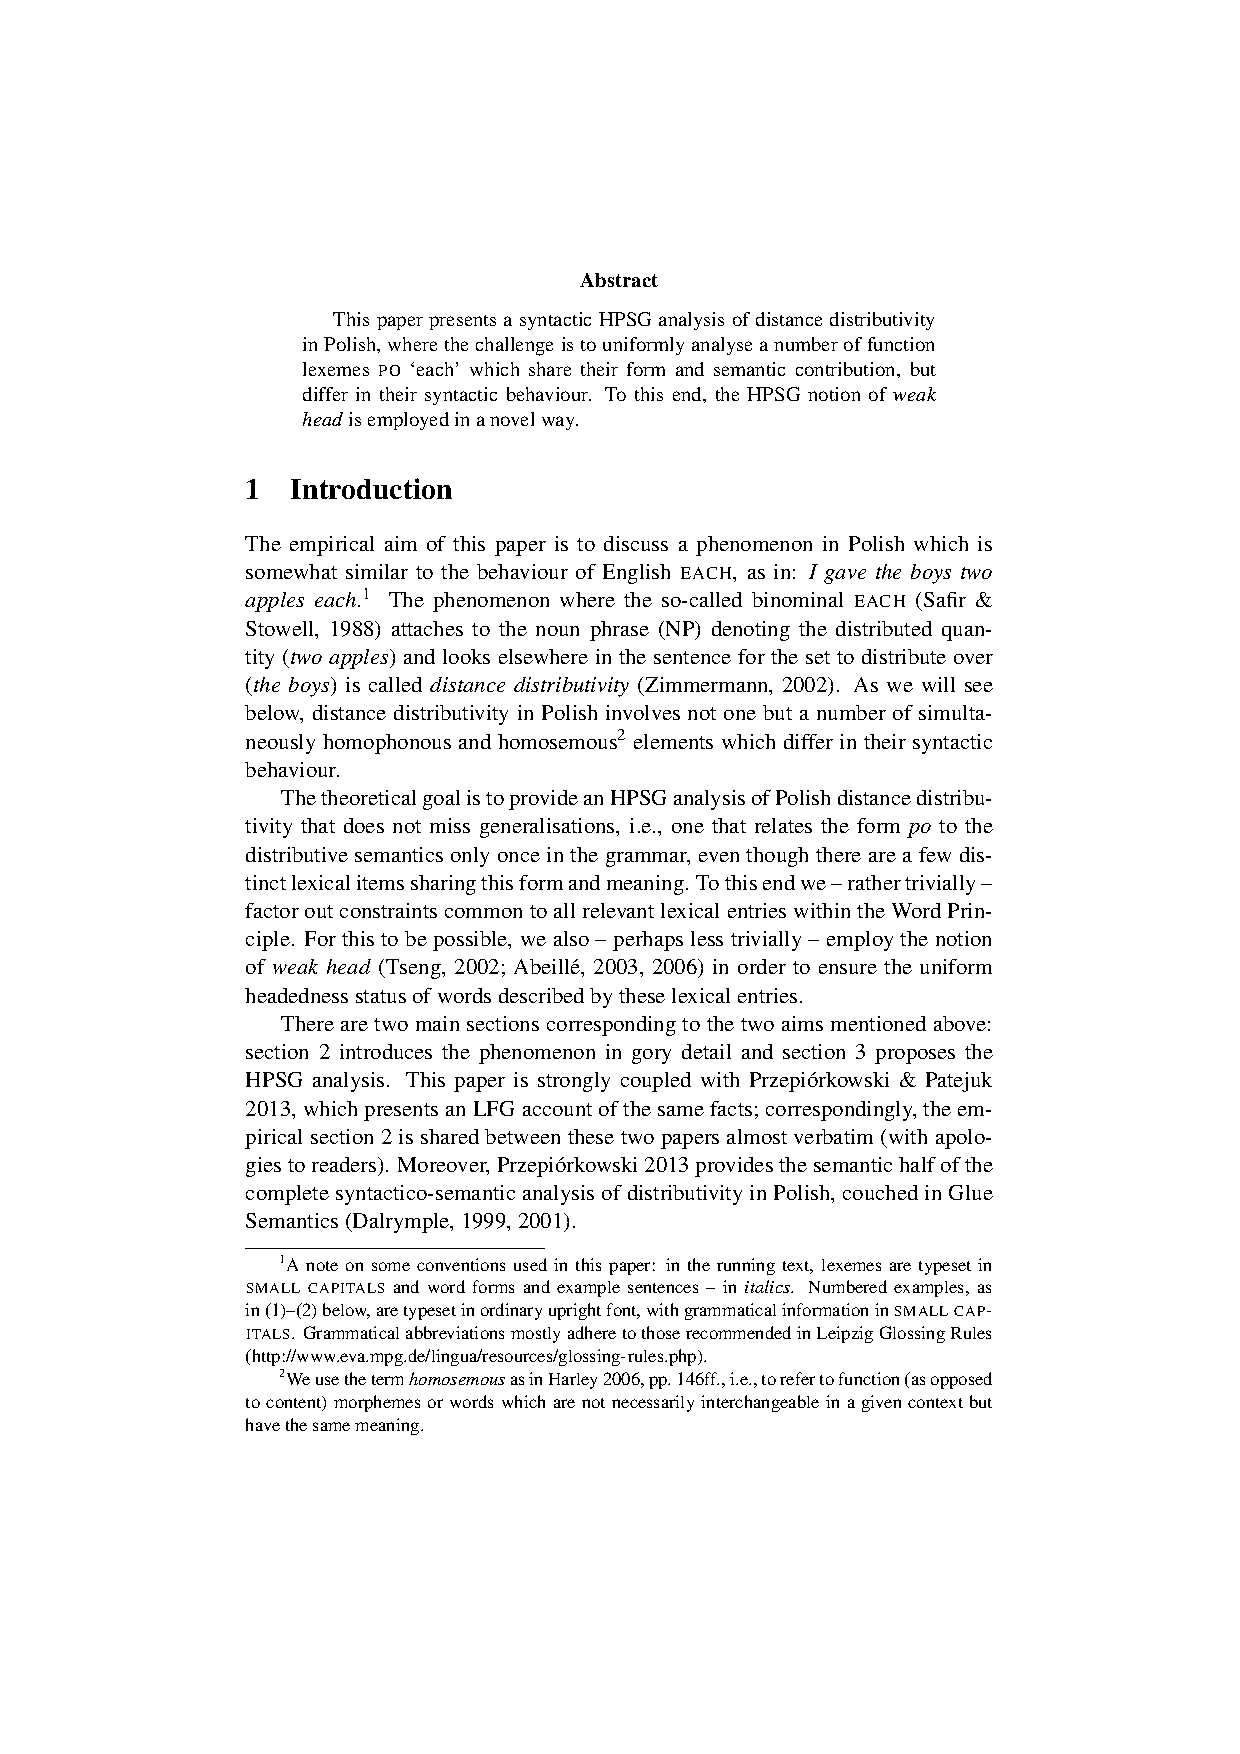
\includepdf[pages=-,pagecommand=\thispagestyle{plain}]{Includes/przepiorkowski.pdf}
        \setcounter{page}{182}
        \phantomsection
        \addcontentsline{toc}{section}{Byong-Rae Ryu: Multiple Case Marking as Case Copying: A Unified Approach to Multiple Nominative and Accusative Constructions in {Korean}}
\thispagestyle{empty}

\begin{center}
  {\huge\bfseries Multiple Case Marking as Case Copying: A Unified Approach to Multiple Nominative and Accusative Constructions in {Korean}\par}

  \bigskip

~\\
\begingroup
\setlength{\leftskip}{0pt plus 1fill}
\setlength{\rightskip}{0pt plus 1fill}
\setlength{\parindent}{0pt}
\setlength{\parfillskip}{0pt}
  \formatauthor{Byong-Rae Ryu}{\begin{tabular}{@{}c@{}}Chungnam National University\end{tabular}}

\par\endgroup

  \vspace*{8ex}

  Proceedings of the 20th International Conference on\par Head-Driven Phrase Structure Grammar

  \bigskip

  Freie Universit\"{a}t Berlin

  \medskip

  Stefan Müller (Editor)

  \medskip

  2013

  \medskip

  CSLI Publications

  \medskip

  pages 182--202

  \medskip

  \url{http://csli-publications.stanford.edu/HPSG/2013}
\end{center}
\vfill

\noindent



\vfill
\noindent
% APA Style
Ryu, Byong-Rae. 2013. Multiple Case Marking as Case Copying: A Unified Approach to Multiple Nominative and Accusative Constructions in {Korean}. In Müller, Stefan (Ed.), \emph{{Proceedings of the 20th International Conference on Head-Driven Phrase Structure Grammar, Freie Universit\"{a}t Berlin}}, 182--202. Stanford,
CA: CSLI Publications. \hfill\href{http://creativecommons.org/licenses/by/4.0/}{\includegraphics[height=.75em]{Includes/ccby.eps}}

\newpage
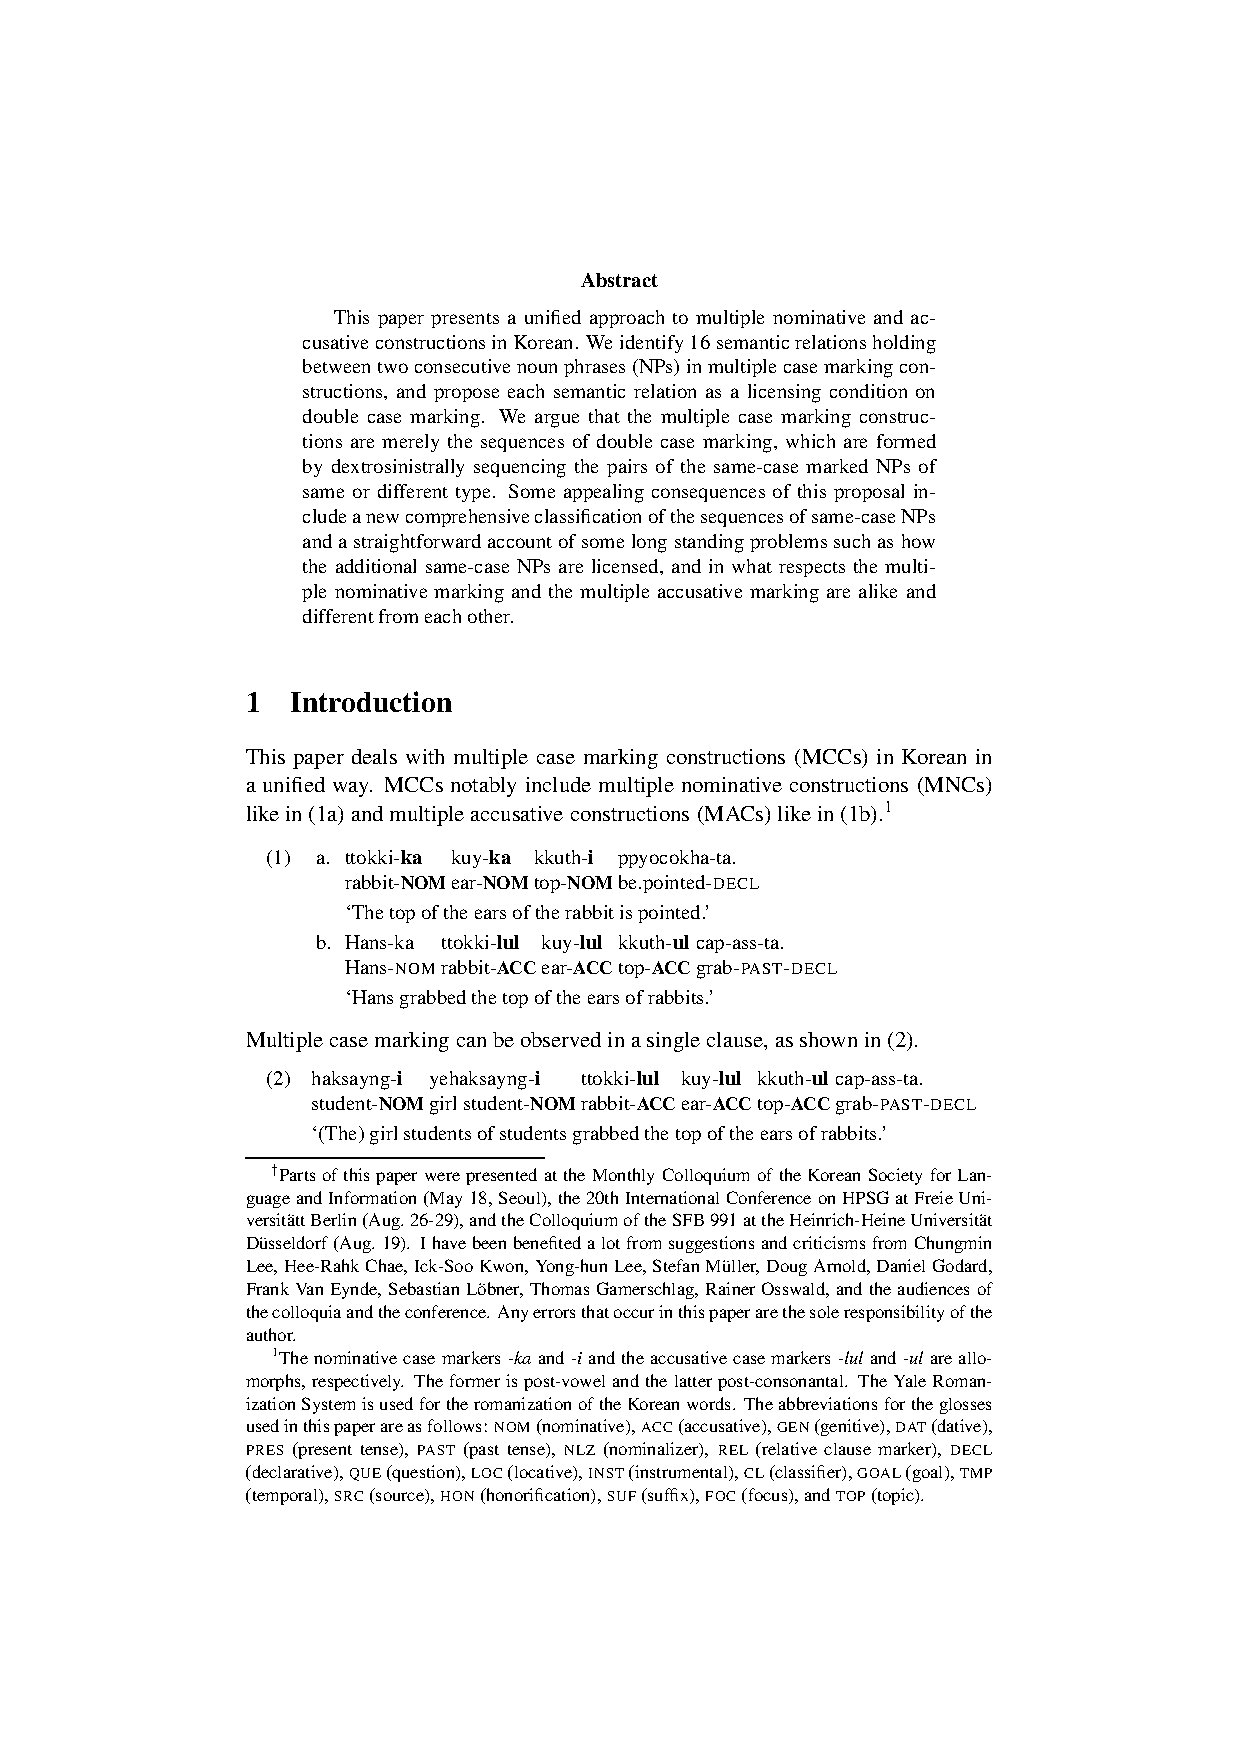
\includepdf[pages=-,pagecommand=\thispagestyle{plain}]{Includes/ryu.pdf}
        \setcounter{page}{203}
        \phantomsection
        \addcontentsline{toc}{section}{Tibor Sz{\'e}cs{\'e}nyi: Argument Inheritance and Left Periphery in {Hungarian} Infinitival Constructions}
\thispagestyle{empty}

\begin{center}
  {\huge\bfseries Argument Inheritance and Left Periphery in {Hungarian} Infinitival Constructions\par}

  \bigskip

~\\
\begingroup
\setlength{\leftskip}{0pt plus 1fill}
\setlength{\rightskip}{0pt plus 1fill}
\setlength{\parindent}{0pt}
\setlength{\parfillskip}{0pt}
  \formatauthor{Tibor Szécsényi}{\begin{tabular}{@{}c@{}}University of Szeged, Hungary\end{tabular}}

\par\endgroup

  \vspace*{8ex}

  Proceedings of the 20th International Conference on\par Head-Driven Phrase Structure Grammar

  \bigskip

  Freie Universit\"{a}t Berlin

  \medskip

  Stefan Müller (Editor)

  \medskip

  2013

  \medskip

  CSLI Publications

  \medskip

  pages 203--221

  \medskip

  \url{http://csli-publications.stanford.edu/HPSG/2013}
\end{center}
\vfill

\noindent



\vfill
\noindent
% APA Style
Szécsényi, Tibor. 2013. Argument Inheritance and Left Periphery in {Hungarian} Infinitival Constructions. In Müller, Stefan (Ed.), \emph{{Proceedings of the 20th International Conference on Head-Driven Phrase Structure Grammar, Freie Universit\"{a}t Berlin}}, 203--221. Stanford,
CA: CSLI Publications. \hfill\href{http://creativecommons.org/licenses/by/4.0/}{\includegraphics[height=.75em]{Includes/ccby.eps}}

\newpage
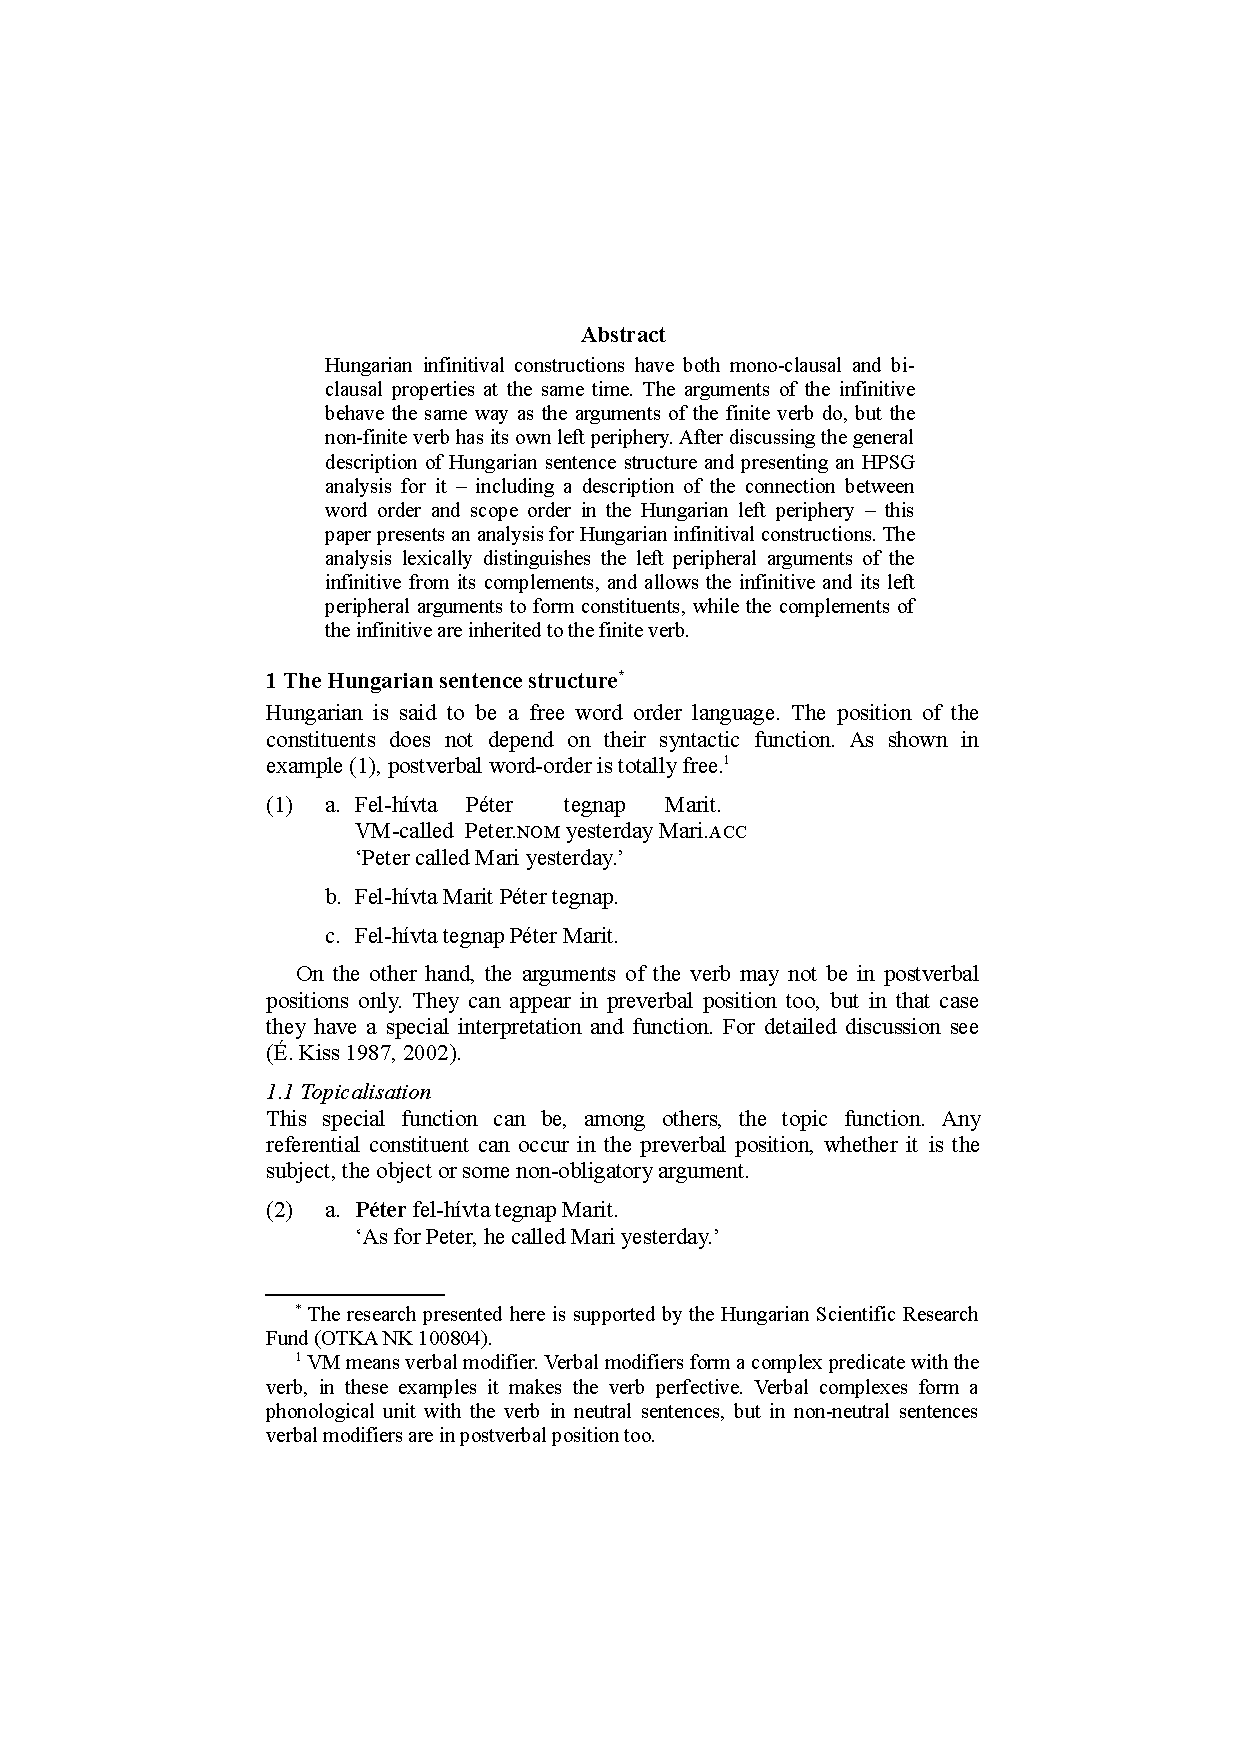
\includepdf[pages=-,pagecommand=\thispagestyle{plain}]{Includes/szecsenyi.pdf}
        \setcounter{page}{222}
        \phantomsection
        \addcontentsline{toc}{section}{Frank Van Eynde, Liesbeth Augustinus: Why and How to Differentiate Complement Raising from Subject Raising in {Dutch}}
\thispagestyle{empty}

\begin{center}
  {\huge\bfseries Why and How to Differentiate Complement Raising from Subject Raising in {Dutch}\par}

  \bigskip

~\\
\begingroup
\setlength{\leftskip}{0pt plus 1fill}
\setlength{\rightskip}{0pt plus 1fill}
\setlength{\parindent}{0pt}
\setlength{\parfillskip}{0pt}
  \formatauthor{Frank Van Eynde}{\begin{tabular}{@{}c@{}}Centre for Computational Linguistics, University of Leuven\end{tabular}}
\formatauthor{Liesbeth Augustinus}{\begin{tabular}{@{}c@{}}Centre for Computational Linguistics, University of Leuven\end{tabular}}

\par\endgroup

  \vspace*{8ex}

  Proceedings of the 20th International Conference on\par Head-Driven Phrase Structure Grammar

  \bigskip

  Freie Universit\"{a}t Berlin

  \medskip

  Stefan Müller (Editor)

  \medskip

  2013

  \medskip

  CSLI Publications

  \medskip

  pages 222--242

  \medskip

  \url{http://csli-publications.stanford.edu/HPSG/2013}
\end{center}
\vfill

\noindent



\vfill
\noindent
% APA Style
Van Eynde, Frank, \& Augustinus, Liesbeth. 2013. Why and How to Differentiate Complement Raising from Subject Raising in {Dutch}. In Müller, Stefan (Ed.), \emph{{Proceedings of the 20th International Conference on Head-Driven Phrase Structure Grammar, Freie Universit\"{a}t Berlin}}, 222--242. Stanford,
CA: CSLI Publications. \hfill\href{http://creativecommons.org/licenses/by/4.0/}{\includegraphics[height=.75em]{Includes/ccby.eps}}

\newpage
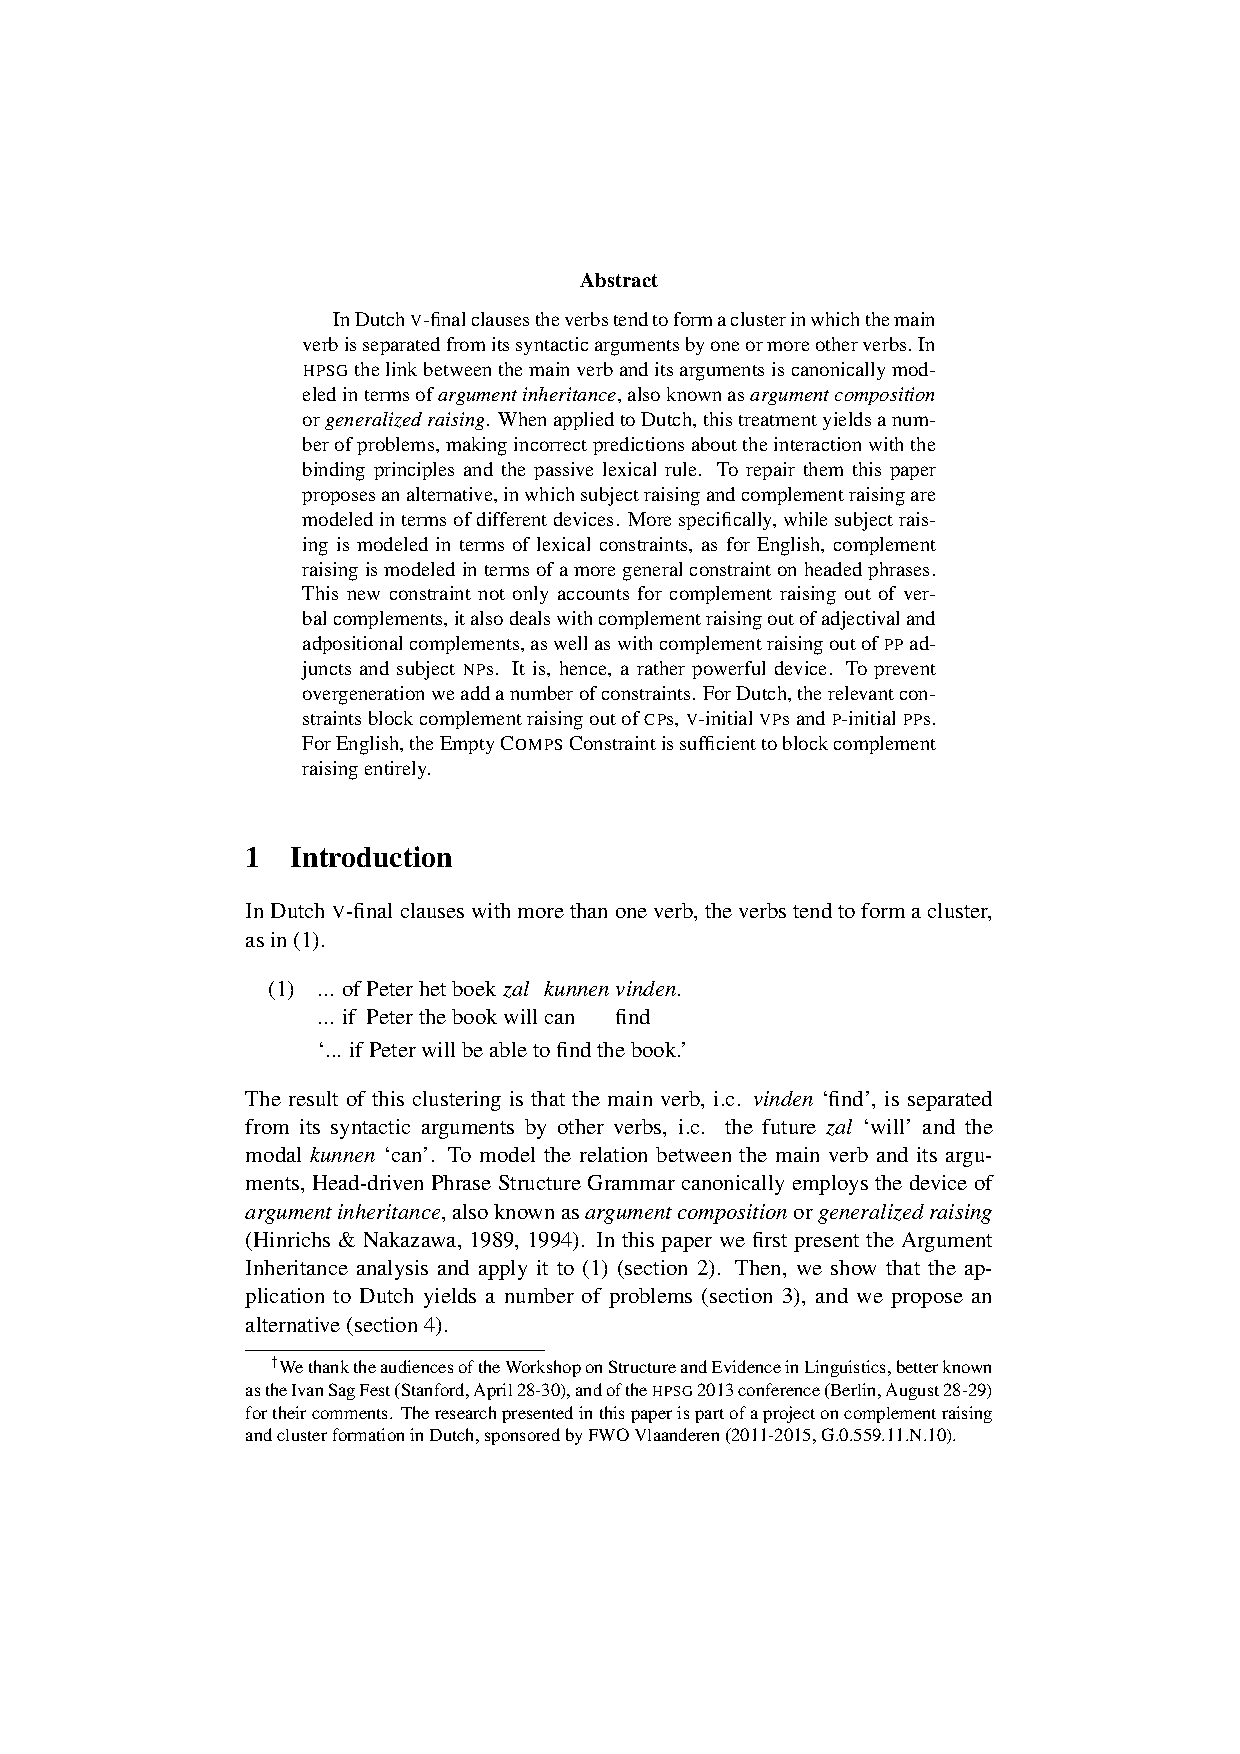
\includepdf[pages=-,pagecommand=\thispagestyle{plain}]{Includes/vaneynde-augustinus.pdf}
\part{Contributions to the Workshop}
\thispagestyle{empty}
\newpage
        \setcounter{page}{244}
        \phantomsection
        \addcontentsline{toc}{section}{Artemis Alexiadou: Where is Non-Active Morphology?}
\thispagestyle{empty}

\begin{center}
  {\huge\bfseries Where is Non-Active Morphology?\par}

  \bigskip

~\\
\begingroup
\setlength{\leftskip}{0pt plus 1fill}
\setlength{\rightskip}{0pt plus 1fill}
\setlength{\parindent}{0pt}
\setlength{\parfillskip}{0pt}
  \formatauthor{Artemis Alexiadou}{\begin{tabular}{@{}c@{}}Universität Stuttgart\end{tabular}}

\par\endgroup

  \vspace*{8ex}

  Proceedings of the 20th International Conference on\par Head-Driven Phrase Structure Grammar

  \bigskip

  Freie Universit\"{a}t Berlin

  \medskip

  Stefan Müller (Editor)

  \medskip

  2013

  \medskip

  CSLI Publications

  \medskip

  pages 244--262

  \medskip

  \url{http://csli-publications.stanford.edu/HPSG/2013}
\end{center}
\vfill

\noindent



\vfill
\noindent
% APA Style
Alexiadou, Artemis. 2013. Where is Non-Active Morphology? In Müller, Stefan (Ed.), \emph{{Proceedings of the 20th International Conference on Head-Driven Phrase Structure Grammar, Freie Universit\"{a}t Berlin}}, 244--262. Stanford,
CA: CSLI Publications. \hfill\href{http://creativecommons.org/licenses/by/4.0/}{\includegraphics[height=.75em]{Includes/ccby.eps}}

\newpage
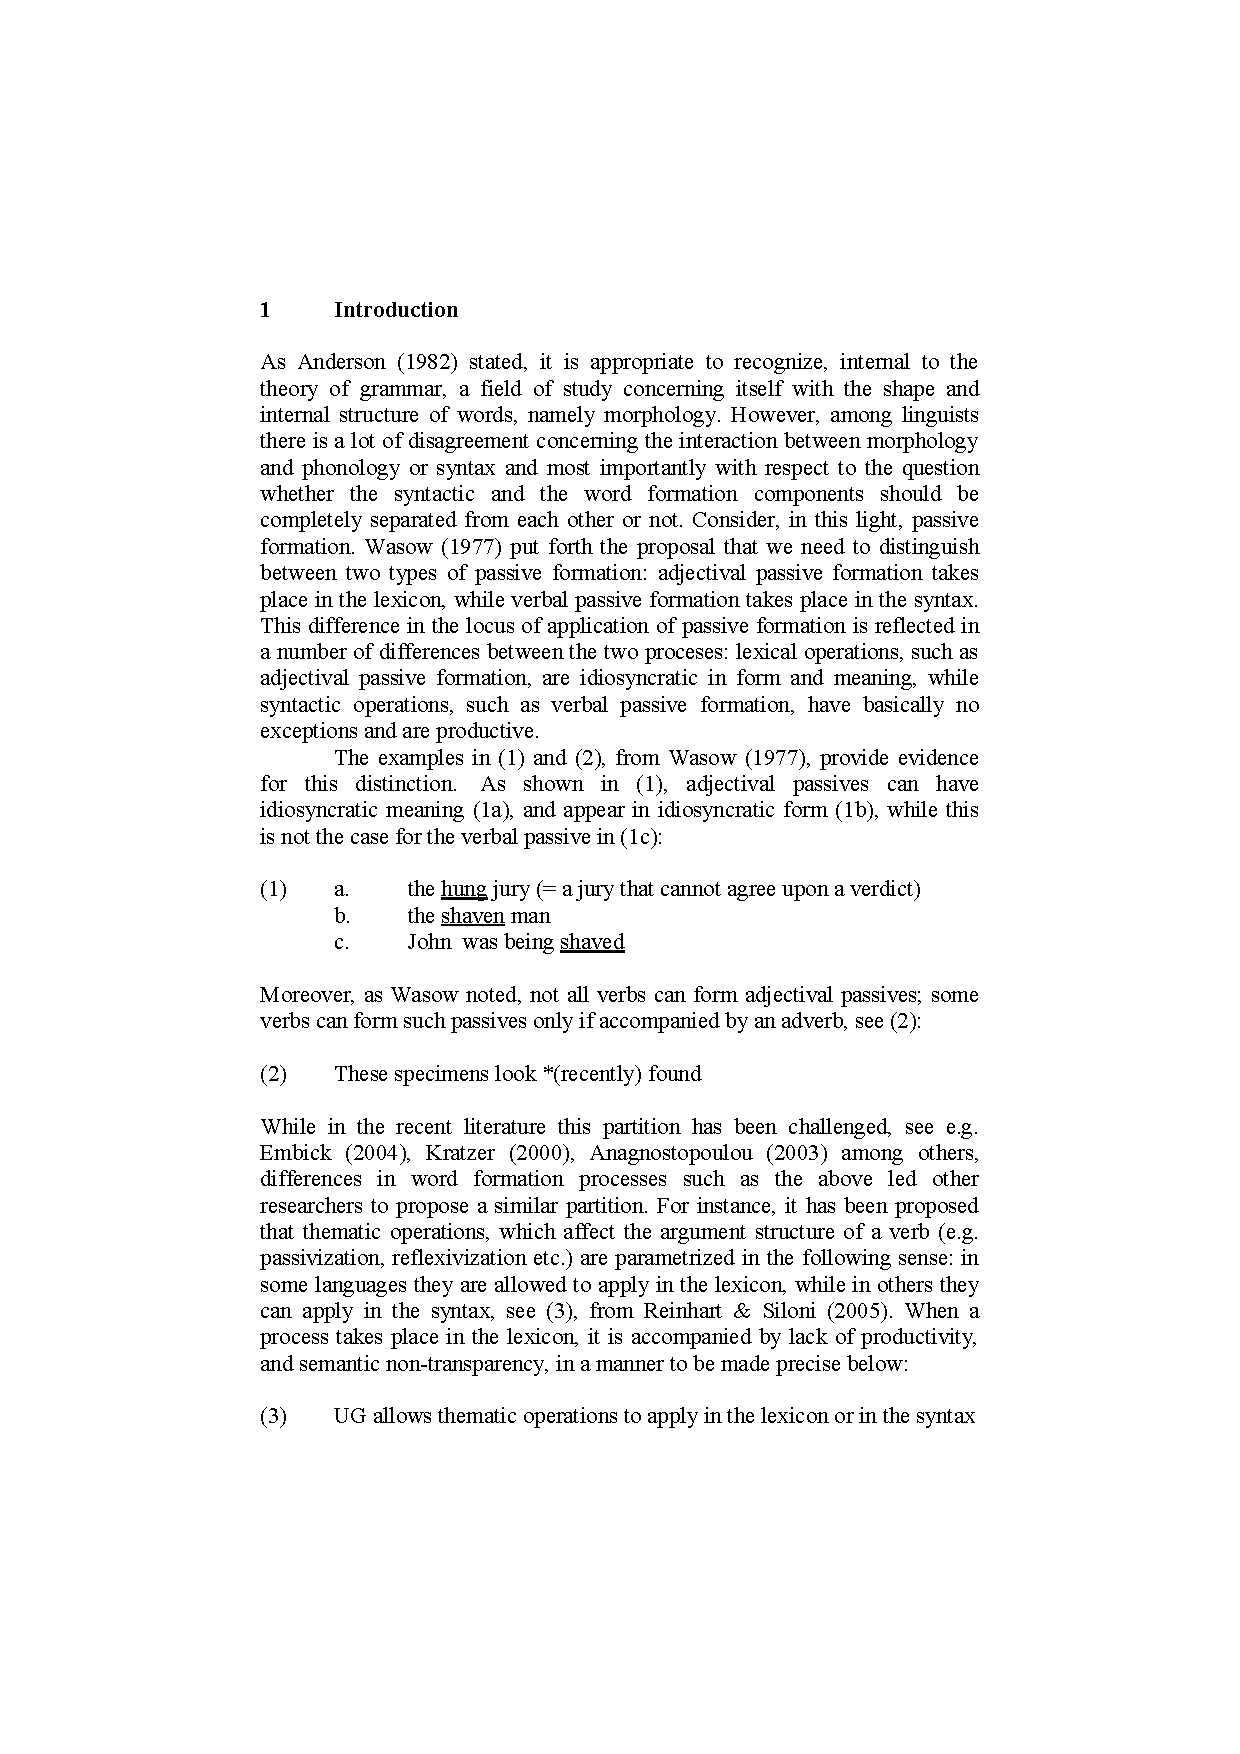
\includepdf[pages=-,pagecommand=\thispagestyle{plain}]{Includes/alexiadou.pdf}
        \setcounter{page}{263}
        \phantomsection
        \addcontentsline{toc}{section}{Peter W. Culicover: {Simpler Syntax} and Explanation}
\thispagestyle{empty}

\begin{center}
  {\huge\bfseries {Simpler Syntax} and Explanation\par}

  \bigskip

~\\
\begingroup
\setlength{\leftskip}{0pt plus 1fill}
\setlength{\rightskip}{0pt plus 1fill}
\setlength{\parindent}{0pt}
\setlength{\parfillskip}{0pt}
  \formatauthor{Peter W. Culicover}{\begin{tabular}{@{}c@{}}The Ohio State University\end{tabular}}

\par\endgroup

  \vspace*{8ex}

  Proceedings of the 20th International Conference on\par Head-Driven Phrase Structure Grammar

  \bigskip

  Freie Universit\"{a}t Berlin

  \medskip

  Stefan Müller (Editor)

  \medskip

  2013

  \medskip

  CSLI Publications

  \medskip

  pages 263--282

  \medskip

  \url{http://csli-publications.stanford.edu/HPSG/2013}
\end{center}
\vfill

\noindent



\vfill
\noindent
% APA Style
Culicover, Peter W. 2013. {Simpler Syntax} and Explanation. In Müller, Stefan (Ed.), \emph{{Proceedings of the 20th International Conference on Head-Driven Phrase Structure Grammar, Freie Universit\"{a}t Berlin}}, 263--282. Stanford,
CA: CSLI Publications. \hfill\href{http://creativecommons.org/licenses/by/4.0/}{\includegraphics[height=.75em]{Includes/ccby.eps}}

\newpage
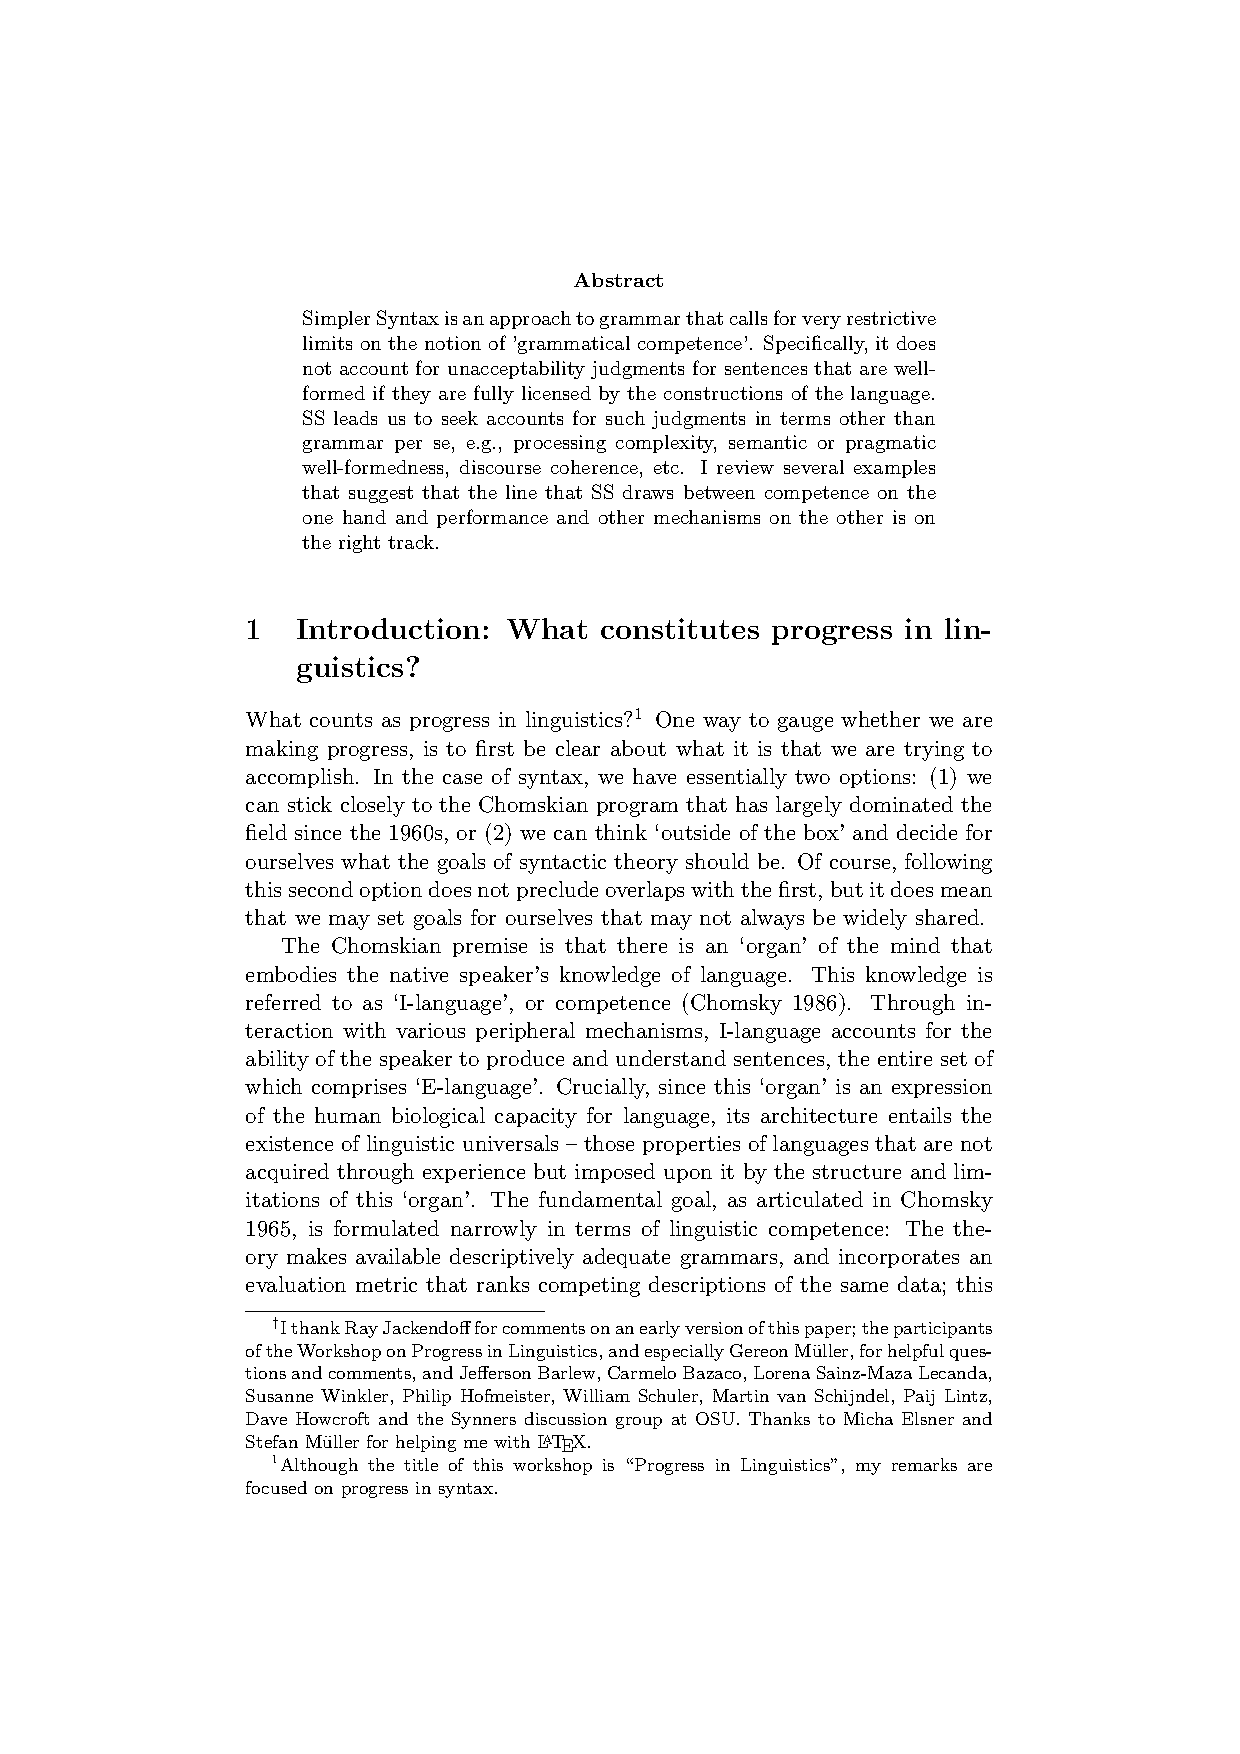
\includepdf[pages=-,pagecommand=\thispagestyle{plain}]{Includes/culicover.pdf}
\end{document}
